% Chapter X

\chapter{Anomaly Detection in Metric Data} % Chapter title
\label{ch:metrics}
\minitoc
\bigskip

Anomaly detection for metric data with various
patterns and data quality has been a great challenge, especially
without labels. Existing anomaly detection algorithms suffer from the hassle of algorithm picking/parameter tuning, heavy reliance on labels, which among other challenges results in large number of false alarms. Metric time series from distributed systems exhibit complex temporal relationships and stochasticity~\cite{donut,fraccaro2016sequential}. 
Accordingly, a possible solution should address both properties. In this chapter, we present a method that captures normal patterns of a time series with an unsupervised anomaly detection model based on VAE (captures stochastic properties) with an RNN as encoder and decoder parts (captures temporal dependence). The observations that deviate from this model of normality are likely to be considered anomalies. 


We summarize the contributions in this chapter, which form a part of a metric anomaly 
10
 detection method, denoted as Metano~\footnote{Parts of this chapter are published in ~\cite{nedelkoski2019anomaly,nedelkoski2020rca,nedelkoski2019edge} and patented in~\cite{nedelkoski2020patent}.}.
\begin{itemize}
\item Model for metric anomaly detection in metric data.
\item Dynamic error threshold approach coupled with a tolerance module to reduce the FP predictions.
\item Anomaly classification module to enrich the description of the anomaly patterns.
\end{itemize}


\begin{figure}[htbp]
\centerline{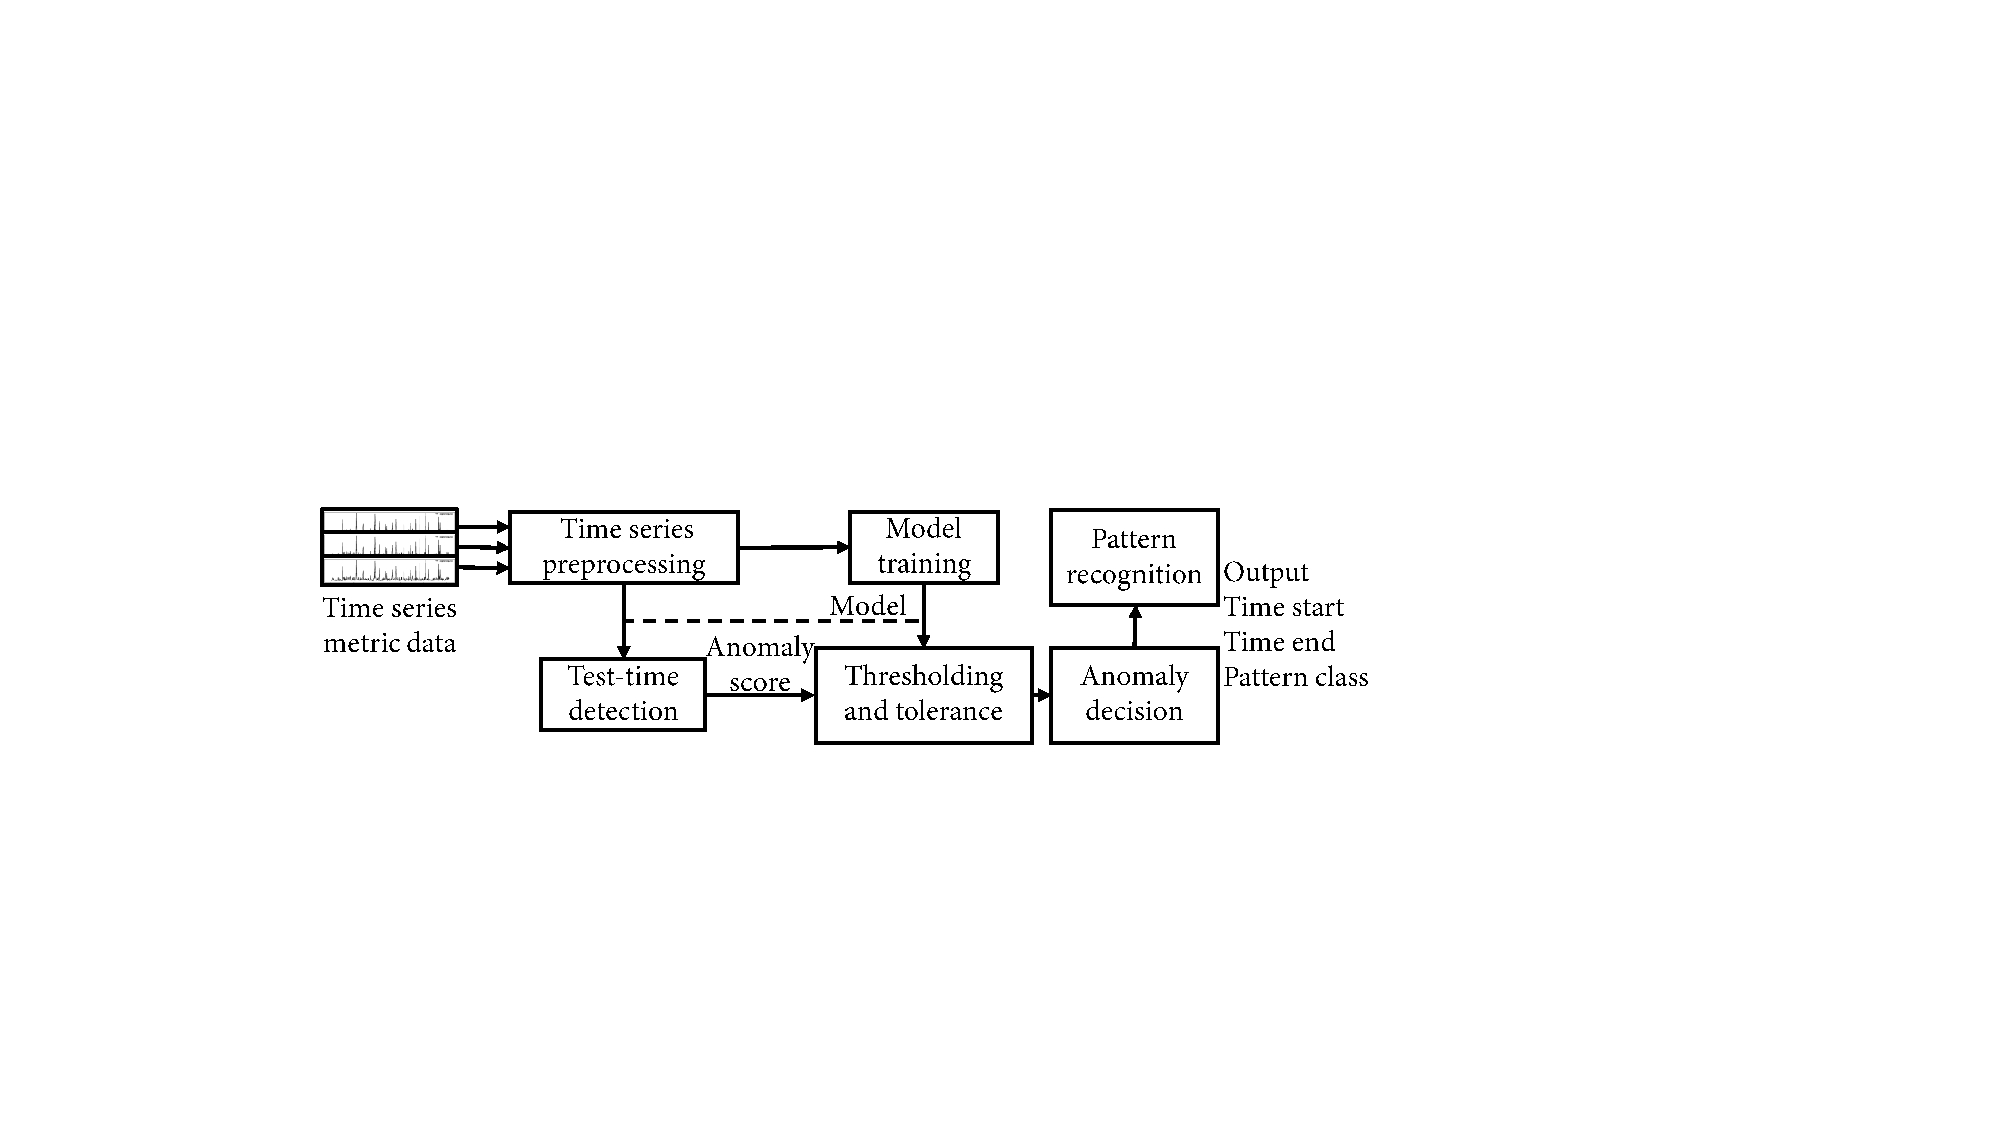
\includegraphics[width=1.0\textwidth]{gfx/chap4/metanooverview.pdf}}
\caption{Overview of Metano.}
\label{fig:metanooverview}
\end{figure}

\section{\textit{Metano}: anomaly detection and classification in metrics}\label{stability}
To formally define Metano, we consider historical observations of a part of a discrete time series representing metric data $\mathbf{x_t} = x_{t-w}, x_{t-w+1}, \dots, x_t$, where $w$ is the size of a defined sliding window over the time series and $x_{t-w}, x_{t-w+1}, \dots, x_t$ are observed values. $\phi(\mathbf{x_t}, \theta): \mathbb{R}^w \rightarrow \mathbb{R}^h \rightarrow [0, a], a \in \mathbb{R}$ is a function represented by a neural network, which maps the input time series window $\mathbf{x_t}$ to a latent representation in $\mathbb{R}^h$, and then to an anomaly score. The method learns the parameters $\theta$, and then, for each incoming instance in the prediction phase $\mathbf{x_1^{test}}, \mathbf{x_2^{test}},\dots, \mathbf{x_i^{test}}, \dots$, predicts whether it is anomalous or normal based on the anomaly scores and threshold $\tau$. If an anomaly is detected, the method classifies it into a finite set of predefined patterns $y_p \in {0, \dots, k}$ with a classifier network $\phi(\mathbf{x_i^{test}}, \hat{\theta})$.

The overall structure of Metano is shown in Figure~\ref{fig:metanooverview}, which consists of two parts, offline training and online (test-time) detection. The time series from the metric data is preprocessed. After the preprocessing, the transformed data are sent to the model training module to learn a model that captures the normal patterns of the time series and outputs an anomaly score for each observation. These anomaly scores are used by the adaptive thresholding and tolerance modules to choose threshold parameters. This offline training procedure can be carried out routinely, e.g., once per day, week, or month. 

The test-time detection module uses the trained model. An observation, $\mathbf{x_{test}}$ at time $t$, after the preprocessing, is predicted by the model to obtain an anomaly score. If the anomaly score passes the checks in the threshold and tolerance module, it will be declared as anomalous; otherwise, it is normal. Parts of the time series that are detected as anomalies are forwarded in the pattern recognition module, where a description of the anomaly will be added. Finally, Metano outputs a dictionary object containing the start timestamp of the window, end timestamp of the window, prediction, and pattern class if the prediction suggests an anomaly. 

\subsection{Time series preprocessing}\label{timeseriespreprocessing}

This step involves two parts, preprocessing in model training and test-time prediction. 
The module starts by querying the $N$ data points of a time series and forwards them into a three-stage pipeline consisting of data cleaning, normalization, and noise reduction. Figure~\ref{fig:preprocessingtimeseries} shows an overview of the preprocessing module.

\begin{figure}[htbp]
\centerline{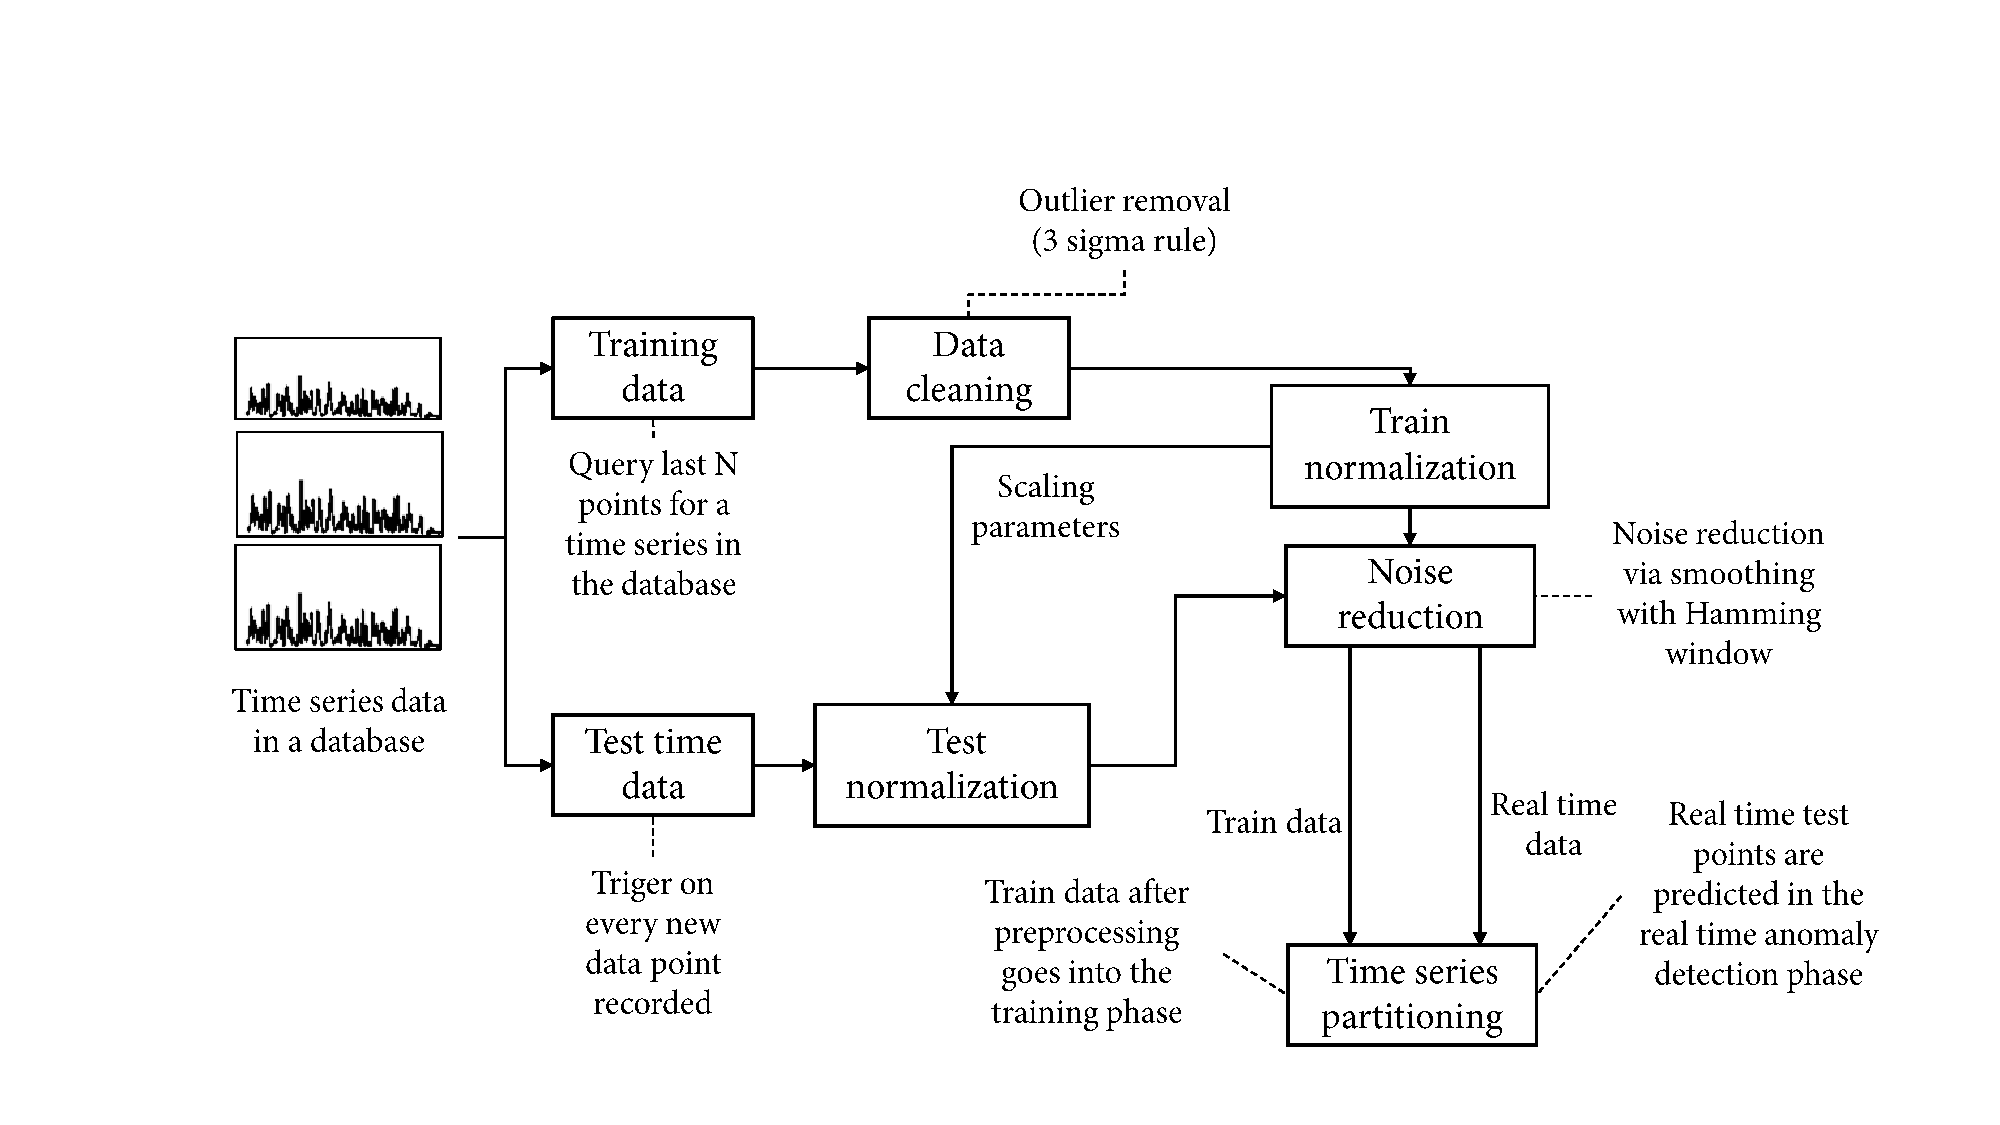
\includegraphics[width=1.0\textwidth]{gfx/chap4/timeseriespreprocessing.pdf}}
\caption{Detailed overview of the time series preprocessing part.}
\label{fig:preprocessingtimeseries}
\end{figure}

In the offline training phase, we perform data cleaning as the first step. Samples having values larger than three standard deviations from the mean are removed from the training batch, according to the three-sigma rule~\cite{pukelsheim1994three}. This is important for robustness and to remove possible anomalies in the training data, as labels are not available. The values are then normalized using min-max scaling (0, 1). Normalization is required and makes the optimization function of the neural network well-conditioned, which is crucial for convergence~\cite{ioffe2015batch}. The min-max normalization is expressed by

\begin{equation}\label{eq8}
\mathbf{x_{t, scaled}} = \frac{\mathbf{x}_t - min(\mathbf{X})}{max(\mathbf{X}) - min(\mathbf{X})},   
\end{equation}

where $min(X)$ and $max(X)$ are saved as scaling parameters and are later used for normalization in the test data. Lastly, in the pipeline, we apply smoothing for noise removal and robustness against small deviations. To this end, the time series is convolved with a Hamming smoothing filter defined with its optimal parameters~\cite{1163506} and size of $M$ as

\begin{equation}\label{eq9}
f(n)=0.54-0.46 \cdot cos\bigg( \frac{2\pi n}{M-1}\bigg), 0 \leq n \leq M-1.
\end{equation}

During the test-time prediction, the time series follows the same preprocessing steps. In the normalization module, $min(X)$ and $max(X)$ are the previously obtained values during the model training part. 
This implies that time series values, which have values larger (smaller) than $max(X)$ ($min(X)$) obtained during the training, will have normalized values larger than 1.0 (smaller than 0.0). 

% \begin{figure}[htbp]
% \centerline{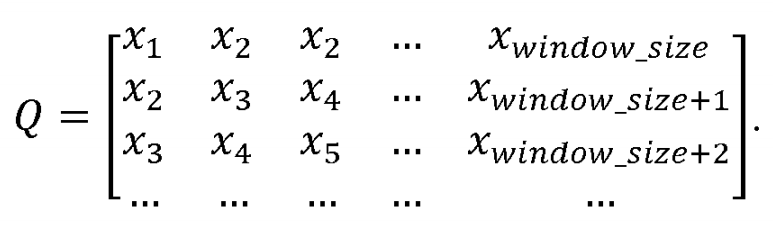
\includegraphics[scale=0.6]{gfx/chap4/splittingtimeseries.png}}
% \caption{Partitioning of a time series with stride=1.}
% \label{fig:timeseriespartitioning}
% \end{figure}

\subsubsection*{Time series partitioning}\label{reshapingtimeseries}
The next step in the pipeline is to transform the time series data into windowed format. In contrast to methods that perform anomaly detection on finite time series data (already windowed, e.g., ECG signals~\cite{acker2017patient}), here we formulate the anomaly detection on sliding windows of the time series, which enables test-time prediction in streaming fashion. Therefore, we define $w$, which is the size of the sliding window. The window is applied to the time series and leads to a training data shape of $(N-w, w, 1)$,

\begin{equation}\label{timeseriespartitioning}
X_{train} = 
\begin{pmatrix}
x_1 & x_2 & \dots & x_{w}\\
x_2 & x_3 & \dots & x_{w+1} \\
\dots \\
x_{N-w} & x_{N-w+1} & \dots & x_{N} \\
\end{pmatrix}_{(N-w) \times w.}
\end{equation}

In the test-time prediction, for each new collected value of the time series, a window of points $x_{test}$ with a size of $w$ is formed, preprocessed, and fed to the network for prediction.

\subsection{Network architecture}
To learn the patterns of the time series data representing the normal system behavior, we design an architecture based on a VAE~\cite{kingma2013auto}, which maps observations (i.e.,input values) to stochastic (i.e., latent) variables, and then reconstructs the input (Figure ~\ref{fig:vae}. The dimensionality of the latent variables is lower than the dimensionality of the input. Therefore, the latent variables are enforced to capture salient features of the normal patterns of the time series.
% These latent variables in VAE are parameters of a known probability distribution (e.g., Gaussian). VAE is a generative model, which learns approximations of the data distributions. 
To detect anomalies, the model uses a window of a time series as an input and performs reconstruction. The reconstruction for normal time series data, similar to those used for model training, is expected to provide a small reconstruction error, as the model is trained by optimizing the error loss function. The reconstruction error for an anomaly sample is expected to be large, as the model is not trained to reconstruct such time series data~\cite{an2015variational}. The decision for anomaly is then based on a threshold on the reconstruction error.

The optimization of VAE relies on variational inference. The variational inference method approximates intractable probability densities through optimization. We consider a probabilistic model with observations $\mathbf{X}=x_{1:n}$, continuous latent variables $\mathbf{z}=z_{1:m}$, and model parameters $\theta$. The task is to compute the posterior distribution

\begin{equation}\label{posterior}
    p(\mathbf{z} \vert \mathbf{X},\theta)=\frac{p(\mathbf{z},\mathbf{X} \vert \theta)}{\int_z p(\mathbf{z},\mathbf{X} \vert \theta)}.
\end{equation}

The computation requires marginalization over the latent variables $\mathbf{z}$, which is intractable. In variational methods, a distribution family is chosen over the latent variables with its variational parameters $q(z_{1:m} \vert \nu)$. The parameters that lead to $q$ as close as possible to the posterior of interest are estimated through optimization~\cite{jordan1999introduction}. However, the true posterior often is not in the search space of the distribution family and thus the variational inference provides only an approximation. 


\begin{figure}[!t]
\centerline{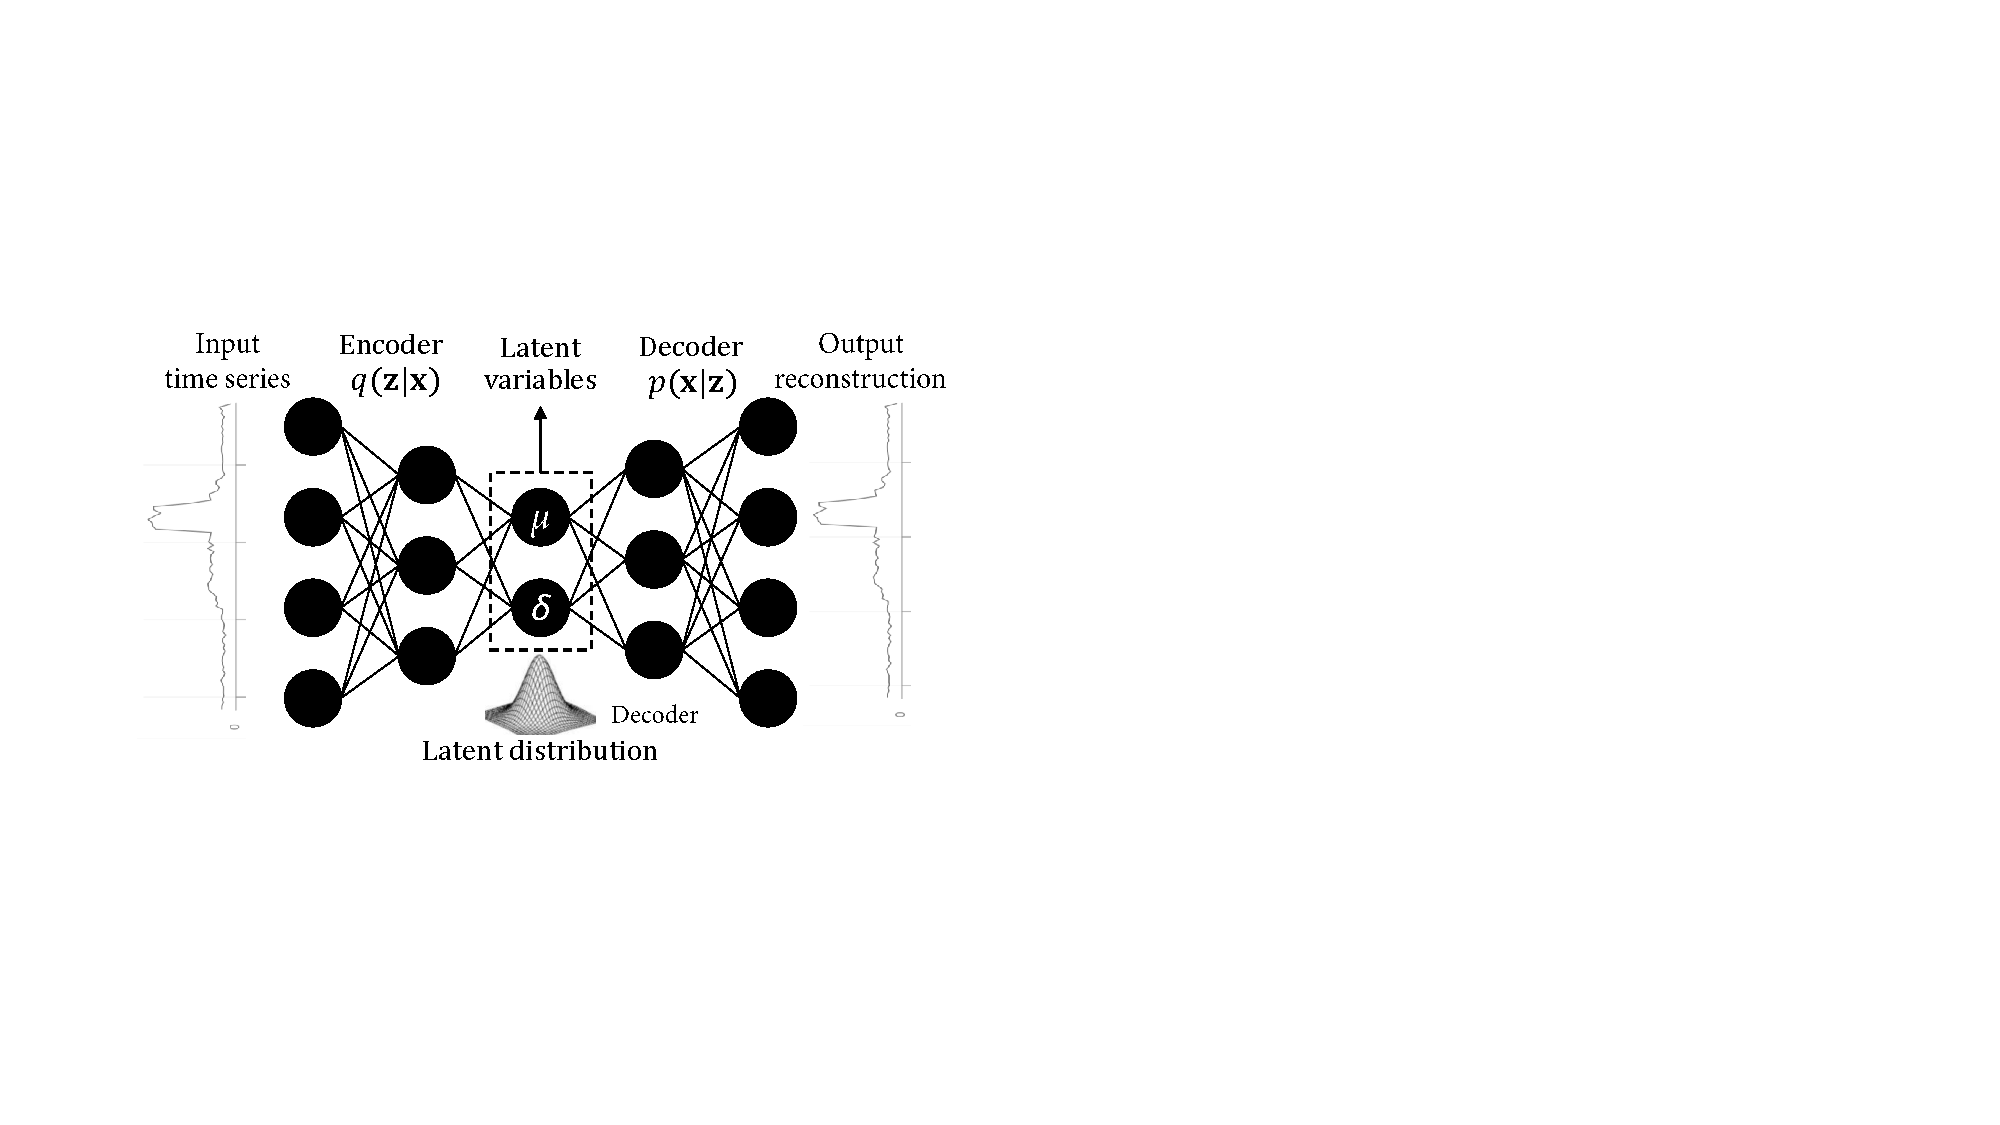
\includegraphics[width=0.7\textwidth]{gfx/chap4/vae.pdf}}
\caption{Architecture of a VAE.}
\label{fig:vae}
\end{figure}


The similarity between the two distributions is measured by the Kullback–Leibler (KL) divergence, a measure of the difference of one probability distribution from a reference probability distribution,

\begin{equation}\label{kl}
    \mathrm{KL}(q \Vert p) = \mathbb{E}_q\left[\log \frac{q(\mathbf{z})}{p(\mathbf{z} \vert \mathbf{x})}\right].
\end{equation}

Direct and exact minimization of the KL divergence is not possible. Instead, as proposed in \cite{jordan1999introduction}, a lower bound on the log-marginal likelihood is constructed,

\begin{align}
    \log p_\theta(\mathbf{x}) \geq \log p_\theta(\mathbf{x}) &- \mathrm{KL}(q(\mathbf{z}\vert \mathbf{x})\Vert p_\theta(\mathbf{z}\vert \mathbf{x})) \label{elbo1} \\ 
    = \mathbb{E}_{q(\mathbf{z} \vert \mathbf{x})}\left[\lambda \log p_\theta(\mathbf{x}|\mathbf{z})\right]
    &- \beta \mathrm{KL}\left[q(\mathbf{z}|\mathbf{x}), p(\mathbf{z})\right] \label{elbo2} \\
    &= \mathrm{ELBO(\mathbf{x})} \nonumber,
\end{align}

where $\lambda$ and $\beta$ are weights in the Evidence Lower Bound (ELBO). In practice, $\lambda=1$ and $\beta$ is slowly annealed to 1 to form a valid lower bound on the evidence~\cite{bowman2015generating}. In VAEs, the ELBO function is optimized by gradient descent using the reparametrization trick, while the parameters of the distributions $p$ and $q$ are obtained by neural networks (encoder and decoder). In Equation~\ref{elbo2}, the first term represents the reconstruction error, while the second corresponds to the regularization. The VAE can only learn the distribution from the windows of the metric time series data. However, it is still not able to recognize temporal dependencies (sequence) in the data.

% The VAE, as described, and shown in Figure~\ref{fig:vae}, is utilized successfully for anomaly detection in metric data from software systems~\cite{donut}. However, owing to the complex temporal dependence of the time series, the anomaly detection is still remains to be a challenging task.

The second property of the time series data that needs to be addressed in the model design is the sequential dependence between values. To preserve the sequential nature of the metric data, in the encoder and decoder parts of the VAE, RNNs are utilized~\cite{rumelhart1986learning}. They are a deterministic type of neural network where the connections between neurons form a directed cycle. This deterministic part of the autoencoder is crucial to capture long-term complex temporal information between the values in the time series observation.


\begin{figure}[!t]
\centerline{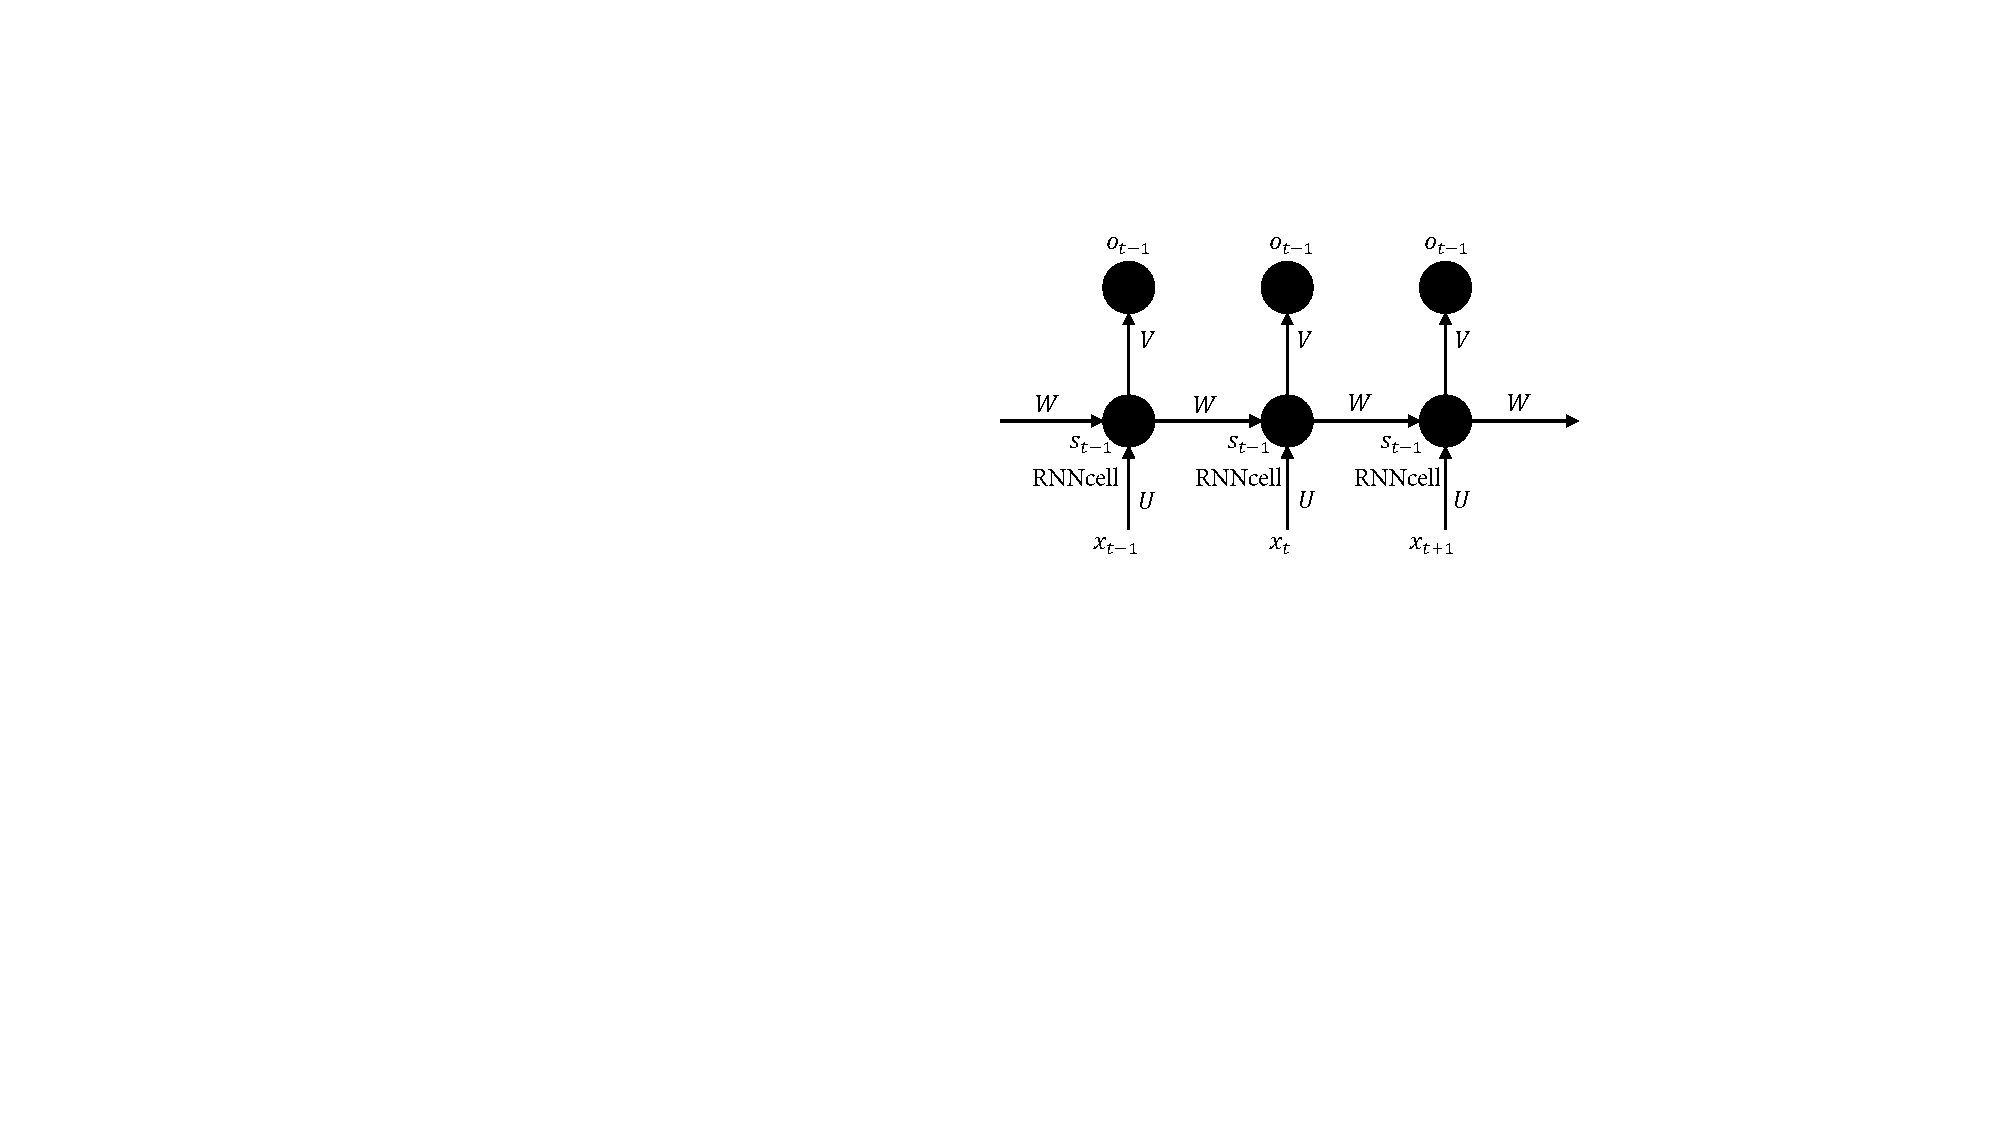
\includegraphics[scale=1.1]{gfx/chap4/rnn.pdf}}
\caption{Architecture of the RNN.}
\label{figrnn}
\end{figure}

In a vanilla RNN, as presented in Figure~\ref{figrnn}, the largest issue is the vanishing gradient problem~\cite{hochreiter1998vanishing}. Numerous solutions exist for this problem, which well perform in practice. The most used RNN types are LSTM~\cite{hochreiter1997long} and GRU~\cite{cho2014properties} cells, which are used in Metano. The GRU cell is a simpler version of the LSTM, which requires less computational resources. The GRU computes an update gate based on the current input vector and hidden state,

\begin{equation}\label{eq4}
  z_t = \sigma(W^{(z)}x_t + U^{(z)}s_{t-1}),
\end{equation}

and then computes the reset game similarly but with different weights,

\begin{equation}\label{eq5}
    r_t=\sigma(W^{(r)}x_t + U^{(r)}s_{t-1}).
\end{equation}

The new memory content is

\begin{equation}\label{eq6}
    \tilde{s_t}=\tanh(Wx_t + r_t \circ U s_{t-1}).
\end{equation}

If the reset gate is 0, this ignores the previous memory and stores only the new information.
The final memory content combines the current and previous timesteps, 

\begin{equation}\label{eq7}
    s_t = z_t \circ s_{t-1} + (1-z_t)\circ \tilde{s_t}.
\end{equation}

The update gate $z$ controls the effect of the past state on the state at timestamp $t$.
If $z$ is close to 1, it can copy information in that unit through numerous time steps. Units with short-term dependencies often have active reset gates. 

This gated flow of the information enables the GRU to model long-term dependencies~\cite{chung2015recurrent}.

We replace the encoder and decoder, i.e., $q(\mathbf{z}|\mathbf{x})$ and $p(\mathbf{x}|\mathbf{z})$, with GRUs (Figure~\ref{fig:vae}. In this regard, we address the stochasticity and temporal dependence in the model design. The overall architecture of the model is shown in Figure~\ref{figmodeltraining} and described below. The objective for model training with gradient descent is Equation~\ref{elbo2}.

\textbf{The input layer} has $w$ units; each of them contains the metric value.

\textbf{The first hidden GRU layer} contains $w/2$ GRU cells for each timestep in the input window. $w/2$ as a hidden dimension size is chosen to restrict and contract the architecture, thus enforcing the hidden states to learn salient features of the time series~\cite{Goodfellow-et-al-2016}. Each of the $w$ input units is fed to the corresponding GRU block. In the first timestep $t=0$, the $0^{th}$ value of the time series is fed. 
The abstract representation learned in the 16 GRU cells, according to Equation~\ref{eq4}-\ref{eq7}, is then propagated to the next timestep $T=1$, where the $1^{st}$ value of the time series of the window is fed, and so on.
We can condition the reconstruction of the next point considering the input of past points. In this regard, in the last timestep, we have an abstract representation of the window of points, which has a salient information for that part of the time series.

\begin{figure}[!t]
\centerline{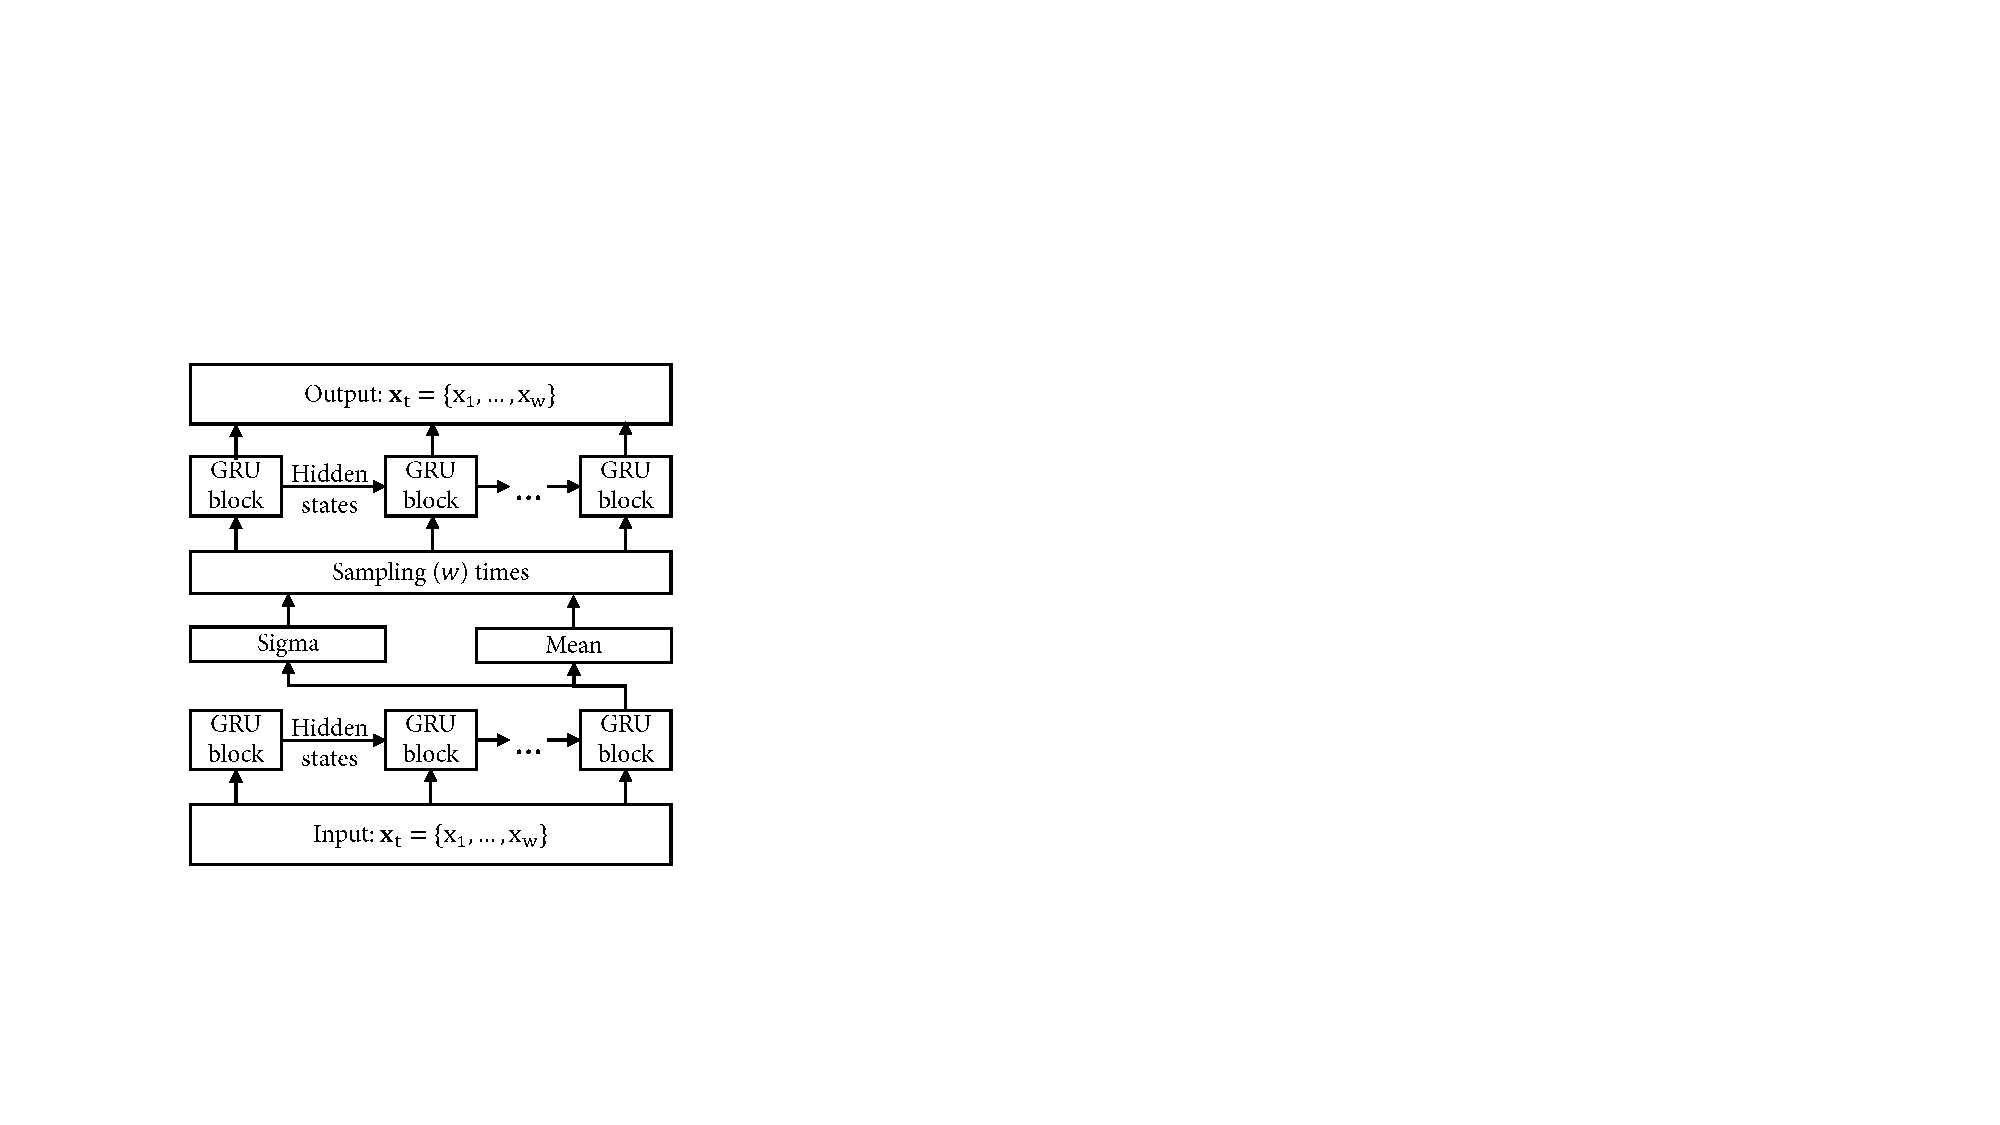
\includegraphics[width=0.5\textwidth]{gfx/chap4/modeltraining.pdf}}
\caption{Model architecture.}
\label{figmodeltraining}
\end{figure}

\textbf{The sampling layer} represents the key part to be able to learn the stochastic process of the time series. This layer is the core part of the VAE and consists of $w/4$ units for the mean and variance of the Gaussian distribution. Gaussian distribution has many beneficial properties, such as analytical evaluation of the KL divergence in the variational loss, and also we can use the reparametrization trick for efficient gradient computation~\cite{kingma2013auto}. It does not matter so much what distribution latent variables follow since using a non-linear decoder can mimic arbitrarily complicated distribution of observations. However, one of the apparent advantages of using the Gaussian in the sampling layer is that it allows easy generation of new samples by sampling in the latent space. 

The model learns the data distributions as an approximation to the multivariate Gaussian. The sampling layer only performs sampling from a multi-variate Gaussian distribution with the learned mean and variance. The complexity of the model allows to learn multiple distributions activated depending on the input.

\textbf{The repeat layer} repeats the sampling layer $w$ times, which needs to be fed into the last hidden GRU layer and utilized for the decoder and reconstruction of the input. This layer is acts like a copy function used for implementation purposes only.

\textbf{Output/GRU layer:} The network uses the output from the previous layer as the input, learns an abstract representation, and, as an output, has the same number $w$ of timesteps, as the output $\mathbf{\hat{x}}$ in autoencoder architectures is the same as the input $\mathbf{x}$. This layer reconstructs the time series.

Through the training of this neural architecture with the loss function of the VAE in Equation~\ref{elbo2} on normal time series data, normal patterns from the data are learned. Once the model of the normality in the system is trained, it can be utilized for anomaly detection by performing reconstructions of the test-time time series.

\subsection{Dynamic error threshold}\label{ch:metrics:sec:metano:subsec:threshold}
The difference between a prediction and observed value of the time series vector is measured by the mean squared error (MSE),

\begin{equation}\label{eqMSE}
MSE=\frac{1}{w}\sum(\mathbf{x_t}-\mathbf{\hat{x_t}})^2.
\end{equation}

Instead of setting a fixed error threshold for anomaly detection, we utilize a validation set (part of the training data) for threshold selection. This is beneficial for the operators and users of Metano, as they do not have to tune and calibrate the threshold in each model training and for every metric. For each window of time series points in the validation set, we apply the model produced by the training set and calculate the MSE between the prediction (reconstruction) and actual sample. At every time step, the errors between the predicted vectors and actual vectors in the validation group are modeled by a Gaussian distribution. We choose the Gaussian distribution to model the MSEs, as per the central limit theorem~\cite{rosenblatt1956central} such samples follow normal distribution.
In the test-time prediction, if the error between reconstructed and observed windows of events (MSE) is within a high level of confidence interval of the above Gaussian distribution, it is considered normal; otherwise, it is considered anomalous.

\subsection{Test-time prediction}
\label{realtimedetectionunstablebehavior}
This module receives data from the preprocessing module described above. The latest model along with the saved training parameters are loaded and used for prediction. For each new value of the time series, the past values forming a window $\mathbf{x_t} = \{x_{t-w}, x_{t-w+1}, ..., x_t\}$ are fed as an input for prediction. The reconstruction error $MSE_{test}$ and probability under the Gaussian distribution of the threshold, obtained during the validation procedure, are computed,

\begin{equation}\label{eqP}
P_{test} = 1 - P(X > MSE_{test}).
\end{equation}


\subsubsection{Tolerance: FP reduction}\label{tolerance}
In large-scale system architectures, a single anomalous point often exists in the time series. However, this does not imply that something is wrong in the particular component. For example, it can be attributed to a small bottleneck in the disk usage or in one of the many components or services. The detection of anomalies having larger impacts enables the DevOps to focus on the most critical potential failures.

We define the tolerance and probability error threshold as parameters. The tolerance represents the allowed number of anomalous windows that have $P_{test}$ larger than the threshold before it flags the whole period as anomalous. In practical scenarios, the tolerance parameter usually is in the range of 1 to 100, but is dependent on the dynamics of the system. The probability outputs $P_{test}$ are kept in a queue with the same size (tolerance) for each new window.  
Each time a new sample is shown to the network to be reconstructed, assigned with the probability of being anomalous, and added to the queue, the tolerance module checks whether the average probability of the samples in the queue

\begin{equation}\label{eqtol}
P_m=\frac{1}{tolerance}\sum_{i}^{tolerance} P_{test(i)},
\end{equation}

is larger than the error threshold. If this is the case, the submodule flags this part of the time series as unstable and reports an anomaly. 
In this regard, we can address the problem of having too many FPs and allow the user to set the sensitivity of the algorithm on his/her demand.
The output of the module is a tuple (first anomaly window timestamp, last anomaly window timestamp).

\subsection{Faulty pattern classification}

Identifying an anomaly without providing insights into its nature is of limited importance. The user may be interested in detecting particular types of anomalies reflected in the time series (incremental, mean shift, gradual increase, cylinder, etc.).  Therefore, we provide a module based on a one-dimensional CNN~\cite{lecun1995convolutional}, which, with a window of the time series as an input, can classify into one of the user-defined patterns described above. The architecture of the CNN consists of a combination of convolutional and max-pooling layers followed by a soft-max layer, which distributes the probability for given pattern. A similar study on time series classification has been recently reported \cite{zhao2017convolutional}.

\begin{figure}[htbp]
\centerline{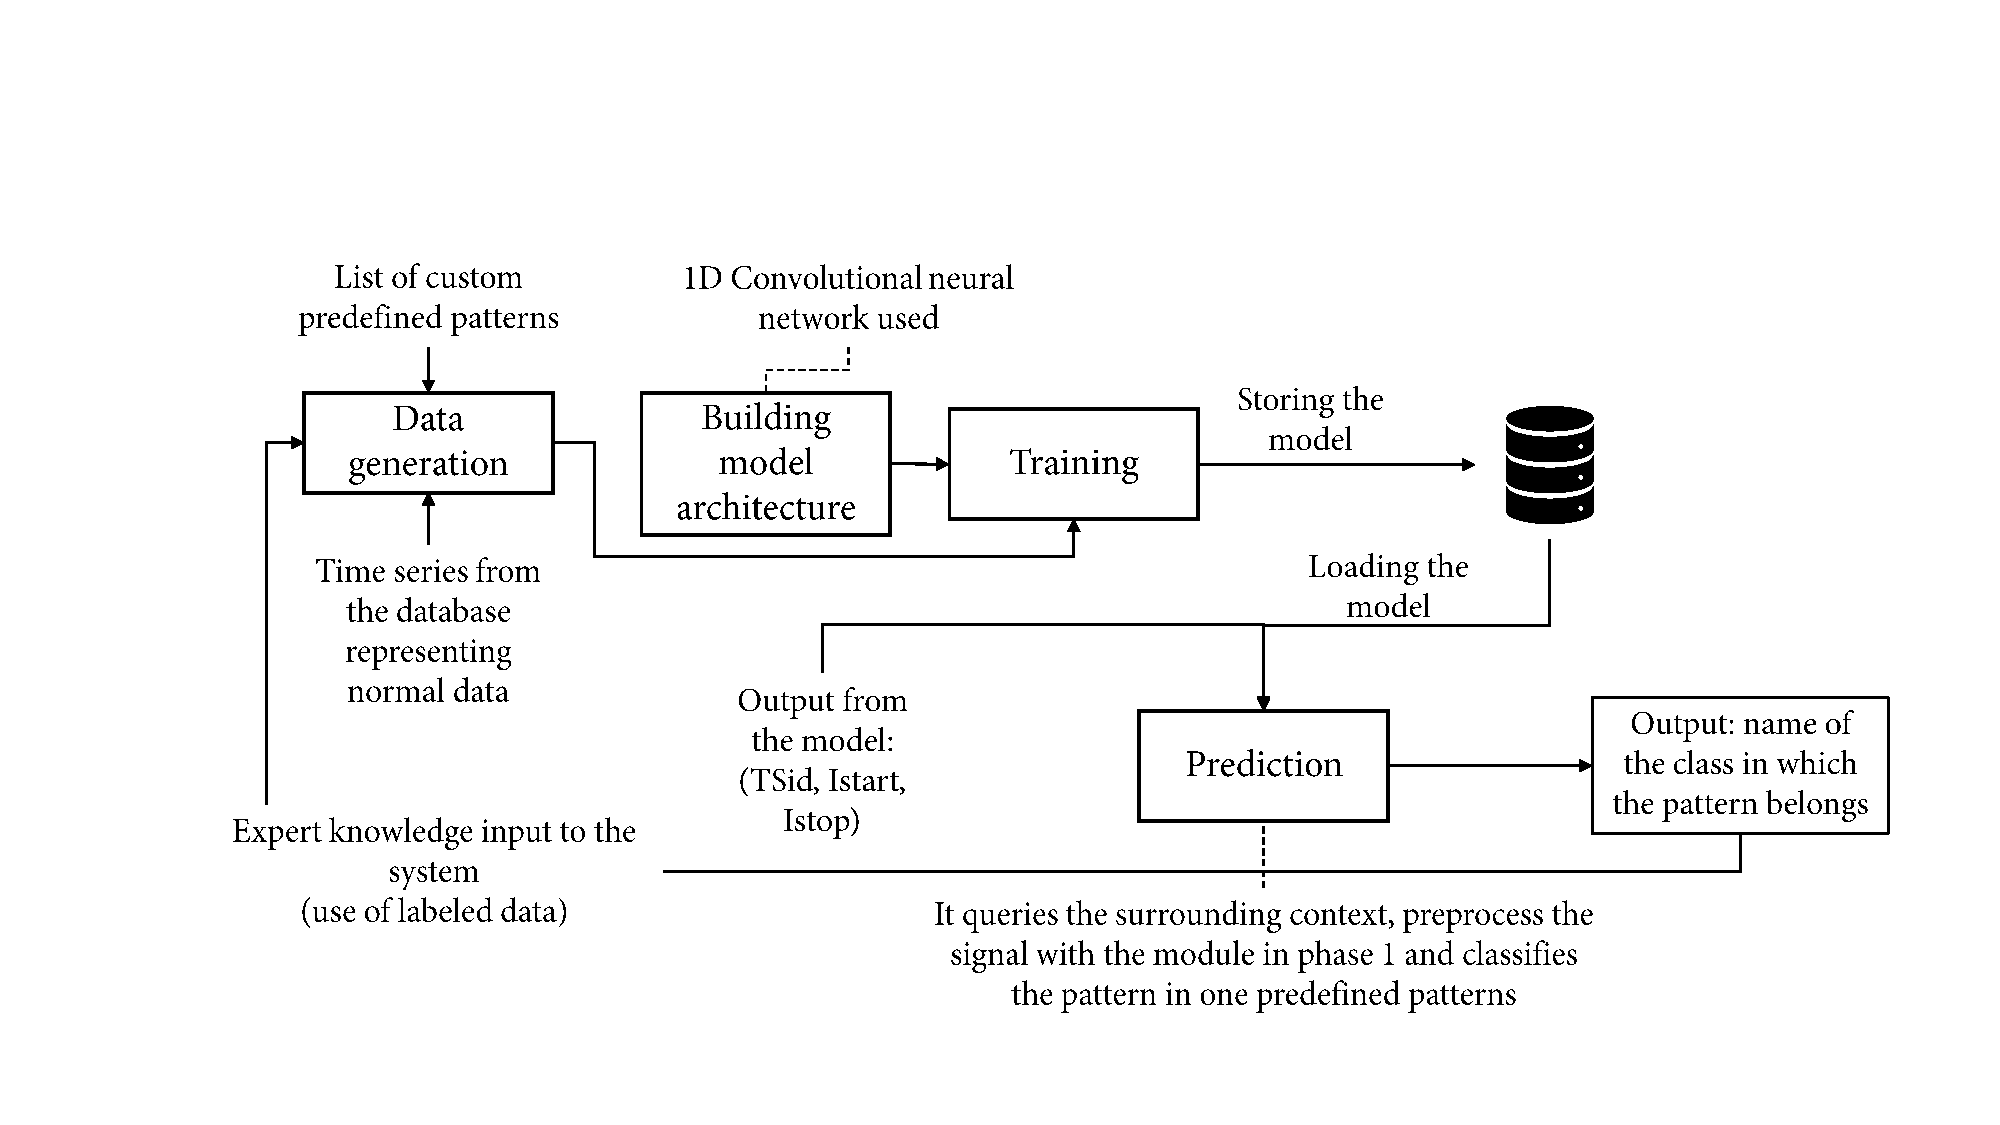
\includegraphics[width=1.0\textwidth]{gfx/chap4/patternclassification.pdf}}
\caption{Anomaly pattern classification.}
\label{fig:patternclassification}
\end{figure}

We show a detailed overview of this module in Figure~\ref{fig:patternclassification}. The data utilized to train the previously described model (see Eq.~\ref{timeseriespartitioning}) are queried and utilized to represent the normal class. The preprocessed normal data are concatenated with the user-defined patterns. These are then fed as an input to the CNN model. 

The model architecture consists of three (convolutional, max-pooling) layers with dropout regularization. The last layer, typical for multi-class classification, is fully connected with the softmax function for computing the probability distribution over the classes. The convolutional networks are naturally invariant to translation, which makes them suitable for faulty pattern detection with a sliding window over the time series. The network is trained using the described data and the model is saved and used for prediction. 

The classifier triggers when the test-time prediction detects an anomaly. The classifier module receives the output from the test-time prediction and requests the particular time series within the provided anomalous time interval. Using the trained model, it maps each sliding window to the predicted class. If the particular pattern is recognized, the module will output the name of the class to which the pattern belongs and will flag the interval as anomalous.

\section{Evaluation}\label{metrics:evaluation}
In this section, we describe three experimental datasets. We then carry out experiments to show the effectiveness and performance of our model. The methods in this chapter are implemented as prototypes in Python using Keras~\cite{chollet2015keras}. The evaluation on the collected datasets was carried out on a regular personal computer with the following specifications: GPU-NVIDIA GTX 1060 6GB, 1TB HDD, 256 SSD, and Intel(R) Core(TM) i7-7700HQ CPU at 2.80 GHz. 
We performed series of experiments to learn the sequence with LSTMs and other deterministic models. The models learned the running mean of the time series. Therefore, we discard comparisons to these methods in this section. In the experiments, Metano is compared to Donut~\cite{donut}, a state-of-the-art univariate metric time series anomaly detection approach based on VAE. 

\subsection{Microservice architecture testbeds}
\begin{figure}[!t]
\centerline{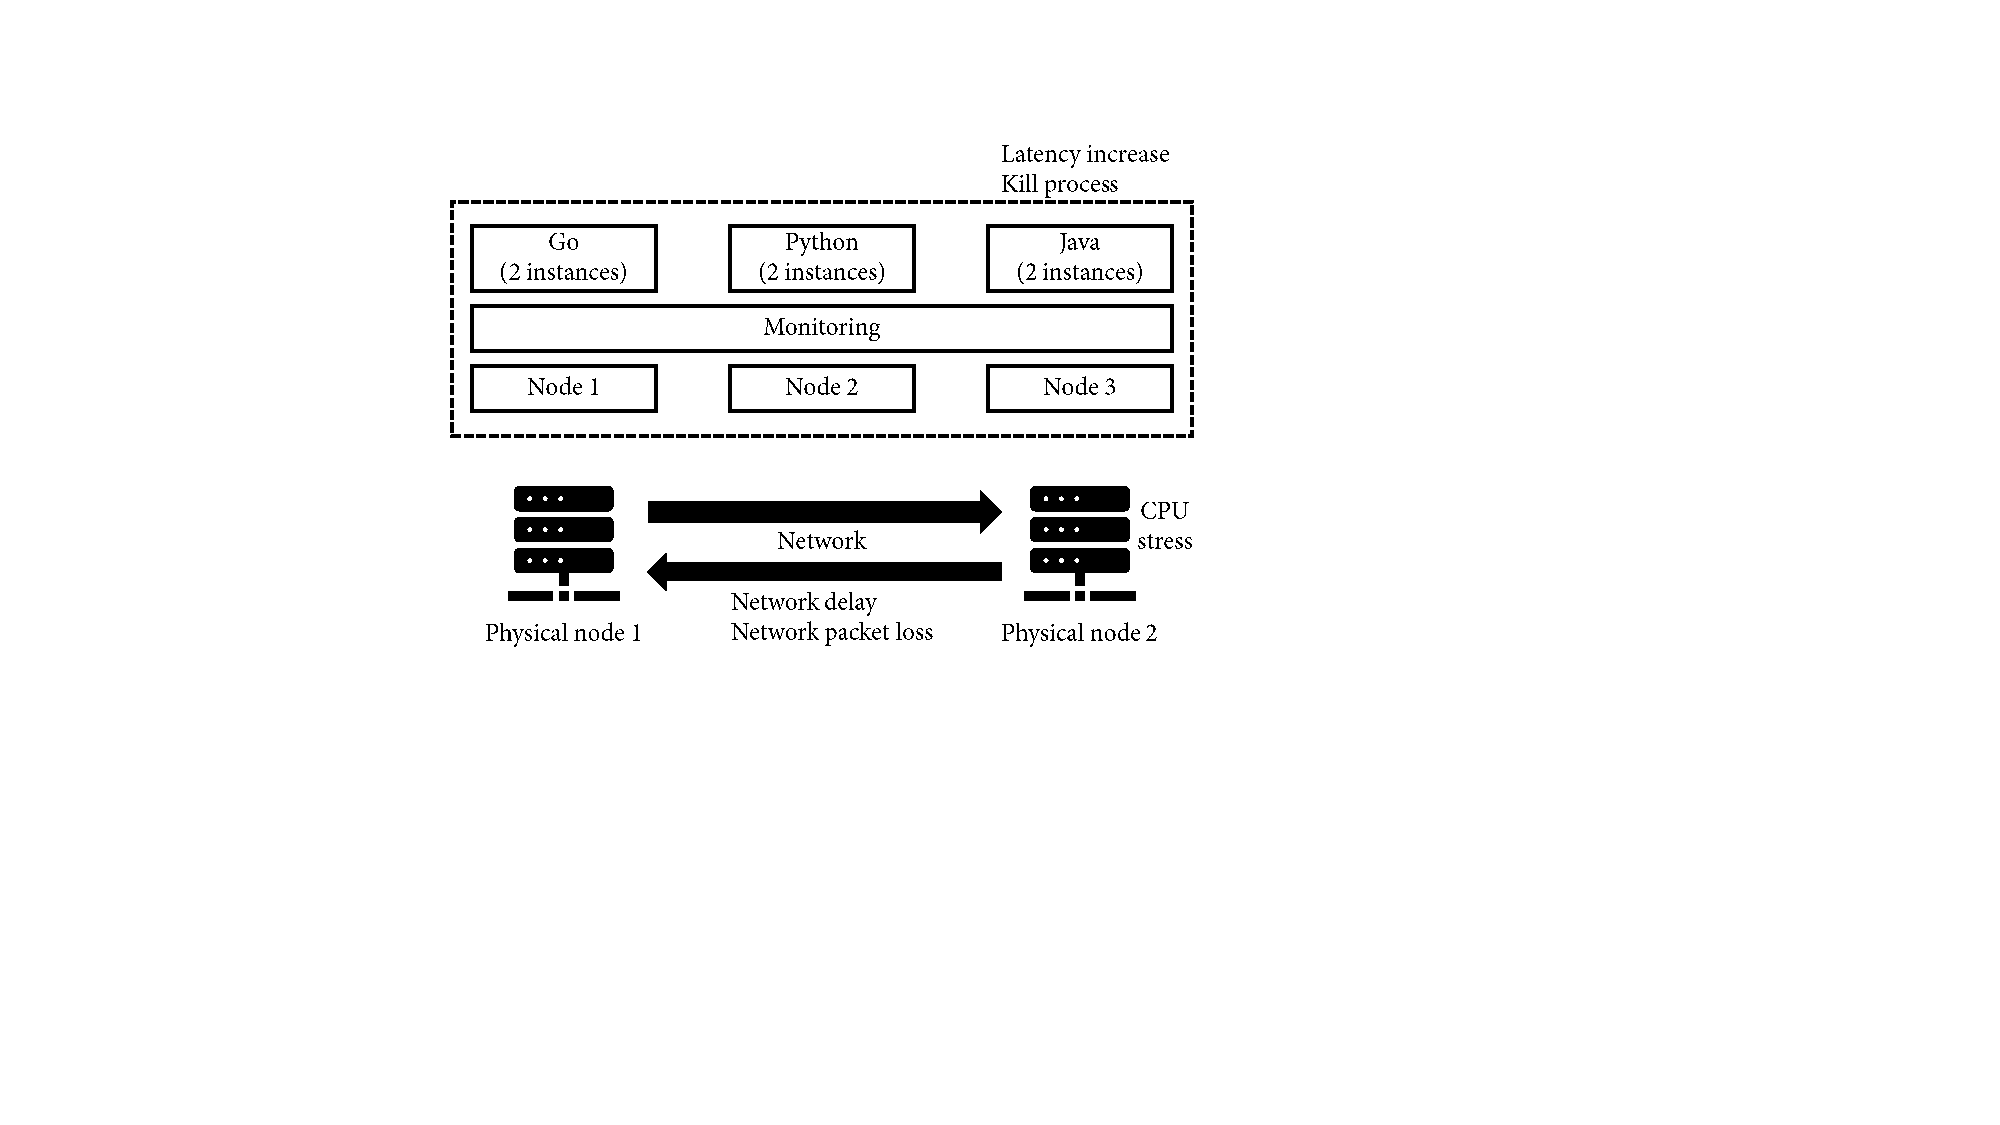
\includegraphics[width=0.8\textwidth]{gfx/chap4/artificialmicroservicetestbed.pdf}}
\caption{Experimental microservice system architecture.}
\label{testbed}
\end{figure}
\textbf{Artificial microservice response times.}
We created an experimental microservice system to evaluate Metano on  representative anomaly scenarios for microservice architectures. For the setup, we used two physical nodes and three virtual machines with enabled tracing, with running instances of Python, Go, and Java applications, respectively. The testbed architecture is shown in Figure~\ref{testbed}. The collected data include the response time metric for each endpoint in the microservice architecture.

To simulate the anomalies, we injected timed physical network anomalies in the form of delay and packet loss, physical node anomalies in the form of CPU stress, and service anomalies in the form of response time increase. They led to six different scenarios on different endpoints in the system, described below. 

\begin{itemize}
    \item Scenario 1: Baseline without anomaly - represents the normal operation (no anomalies) of the system and is used to train the detection algorithms.
    \item Scenario 2: Service latency increase - profile 1 (injection of latency (1 s) for a duration of 15 s).
    \item Scenario 3: Service latency increase - profile 2 (injection of latency (1, 5, 30 s) for a duration of 30 s, 1 min, and 10 min on nodes 1,2,3).
    \item Scenario 4: Network packet loss - A packet loss (10\%, 20\%, 30\%) is injected on one of the network links for durations of 1, 5, and 10 min. 
    \item Scenario 5: Network delay - A network delay (1, 2, 3 s) is injected on the network for durations of 1, 5, and 10 min.
    \item Scenario 6: Server process dies -  One process is killed on nodes 1 and 3 for durations of 1, 5, and 10 min.
\end{itemize}


\textbf{Response times from production-cloud data.}
Even in small controlled experimental setups, the noise is high and the time series changes rapidly over time. This already poses challenges for the anomaly detection algorithm. However, testing the approach on large-scale production cloud data is required to show the viability of the approach.

The dataset contains response times of three main services for a period of four days, obtained from a large-scale production cloud. 
The signal-to-noise ratio in the data is small as numerous components affect the response time of microservices. The time series evolves faster and changes its distribution over time while having a stochastic behavior. The time series of the response time from one of the production services was already plotted and discussed in~\autoref{ch:concepts:sec:anomalydetectionindistributedsoftwaresystems:subsec:metric}.

\textbf{Sockshop microservice testbed.} In addition to the artificially created microservice architecture testbed, we set a second testbed on Google Cloud Engine\footnote{https://cloud.google.com/compute} where we run the Sock-shop\footnote{https://microservices-demo.github.io/} microservice benchmark consisting of seven microservices. The monitoring tools include node-exporter\footnote{https://github.com/prometheus/node\_exporter}, Cadvisor\footnote{https://github.com/google/cadvisor}, and Prometheus\footnote{https://prometheus.io}. Sock Shop simulates the user-facing part of an e-commerce website, which sells socks. It is intended to aid the demonstration and testing of microservice and cloud native technologies. We also developed a workload generator to send requests to different services. To inject the performance issues in microservices, we customize the Docker images of the services by installing the fault injection tools. Three types of faults were injected into the Sock shop services, (1) network anomalies by increasing the latency, (2) CPU hog, and (3) memory leak, by exhausting the CPU and memory resources in the container with stress-ng. For each anomaly, we repeated the experiments multiple times in the duration of at least 2 min. To train the model, we collect data for 1 h in the normal status. The data include a total of seven metrics for each service (CPU, memory, and network usage, on host and container levels, and service response time).


% Out of them, we selected three services of interest. 
% The anonymized names along with the count of the samples is given in Table \ref{tableclusters}

% \begin{table}[!t]
% \centering
% \caption{Ser for analysis.}
% \begin{tabular}{ll}\hline
% ClusterID		&Count\\ \hline
% \{host\}/v1/\{p\_id\}/cs/limits		&12900\\
% \{host\}/v1/\{t\_id\}/cs/delete		&2732\\
% \{host\}/v2/\{t\_id\}/servers/detail		&6468\\
% \hline 
% \end{tabular}
% \label{tableclusters}
% \end{table}


\begin{table}[htbp]
\centering
\caption{Metano: F1 scores for 15 endpoints in five anomaly scenarios of the experimental testbed data.}
\resizebox{1.0\textwidth}{!}{%
\begin{tabular}{l|cc|cc|cc|cc|cc}
\hline
\multicolumn{1}{c|}{Scenario}                                 & \multicolumn{2}{c|}{S2} & \multicolumn{2}{c|}{S3} & \multicolumn{2}{c|}{S4} & \multicolumn{2}{c|}{S5} & \multicolumn{2}{c}{S6} \\ \hline
\begin{tabular}[c]{@{}l@{}}Endpoint ID/\\ Method\end{tabular} & Donut      & Metano     & Donut      & Metano     & Donut      & Metano     & Donut      & Metano     & Donut      & Metano     \\ \hline
1                                                             & -          & -          & 0.85       & 0.85       & 0.93       & 0.95       & 0.95       & 0.98       & 0.99       & 0.99       \\
2                                                             & -          & -          & -          & -          & 0.99       & 0.99       & 0.93       & 0.98       & -          & -          \\
3                                                             & -          & -          & -          & -          & 0.98       & 0.96       & 0.98       & 0.99       & 0.97       & 0.96       \\
4                                                             & -          & -          & 0.90       & 0.99       & -          & -          & -          & -          & -          & -          \\
5                                                             & -          & -          & -          & -          & 1.0        & 1.0        & 0.95       & 0.98       & 0.97       & 0.97       \\
6                                                             & -          & -          & 0.93       & 0.98       & -          & -          & -          & -          & 0.81       & 0.86       \\
7                                                             & -          & -          & 0.96       & 0.95       & 0.96       & 0.98       & 0.92       & 0.97       & -          & -          \\
8                                                             & -          & -          & 0.98       & 0.98       & -          & -          & -          & -          & -          & -          \\
9                                                             & -          & -          & 0.88       & 0.92       & 0.92       & 0.91       & 0.99       & 0.99       & 1.0        & 1.0        \\
10                                                            & 0.85       & 0.90       & 0.87       & 0.95       & 0.93       & 0.95       & 0.92       & 0.99       & 0.94       & 0.98       \\
11                                                            & -          & -          & 0.96       & 0.96       & -          & -          & -          & -          & -          & -          \\
12                                                            & 0.89       & 0.85       & -          & -          & 0.79       & 0.83       & 1.0        & 0.99       & 0.95       & 0.97       \\
13                                                            & 0.90       & 0.95       & 0.91       & 0.98       & -          & -          & 0.91       & 0.94       & 0.96       & 0.99       \\
14                                                            & 0.91       & 0.99       & 0.87       & 0.95       & -          & -          & -          & -          & 0.94       & 0.98       \\
15                                                            & -          & -          & 0.86       & 0.97       & 0.95       & 0.95       & 0.99       & 0.98       & 1.0        & 1.0        \\ \hline
\end{tabular}\label{table_res_vae}
}
\end{table}
\subsection{Results and discussion}




\noindent\textbf{Artificial microservices response times.}
The F1 scores of Metano and Donut are shown in Table~\ref{table_res_vae} for all 15 endpoints in our experimental testbed across the five different scenarios. The number of injected anomalies depends on each scenario and endpoint. The missing values in Table~\ref{table_res_vae} imply that the anomaly did not affect those endpoints. 

Notably, the described approach in this chapter is comparable to or outperforms Donut~\cite{donut}. Overall, the results in the table and figure indicate that the combination of generative models, such as the VAE with GRU units, that extract temporal information is effective. The method generalizes over different anomaly scenarios. The highest scores are observed in S5 and S6, where the anomalies are most reflected in the values.

In Figure~\ref{scenarios}, scenarios 5 and 6 are illustrated, where the method successfully flags the majority of anomalous values. The method successfully flags almost all anomalous events. False positives are observed only around the 800-th and 1250-th data points of the time series, where the response time is increased owing to the considerable noise. 

Overall, the method performs comparably well, successfully handling variety of anomalies.
\begin{figure*}[!t]
     \centering
     \subfloat[][]{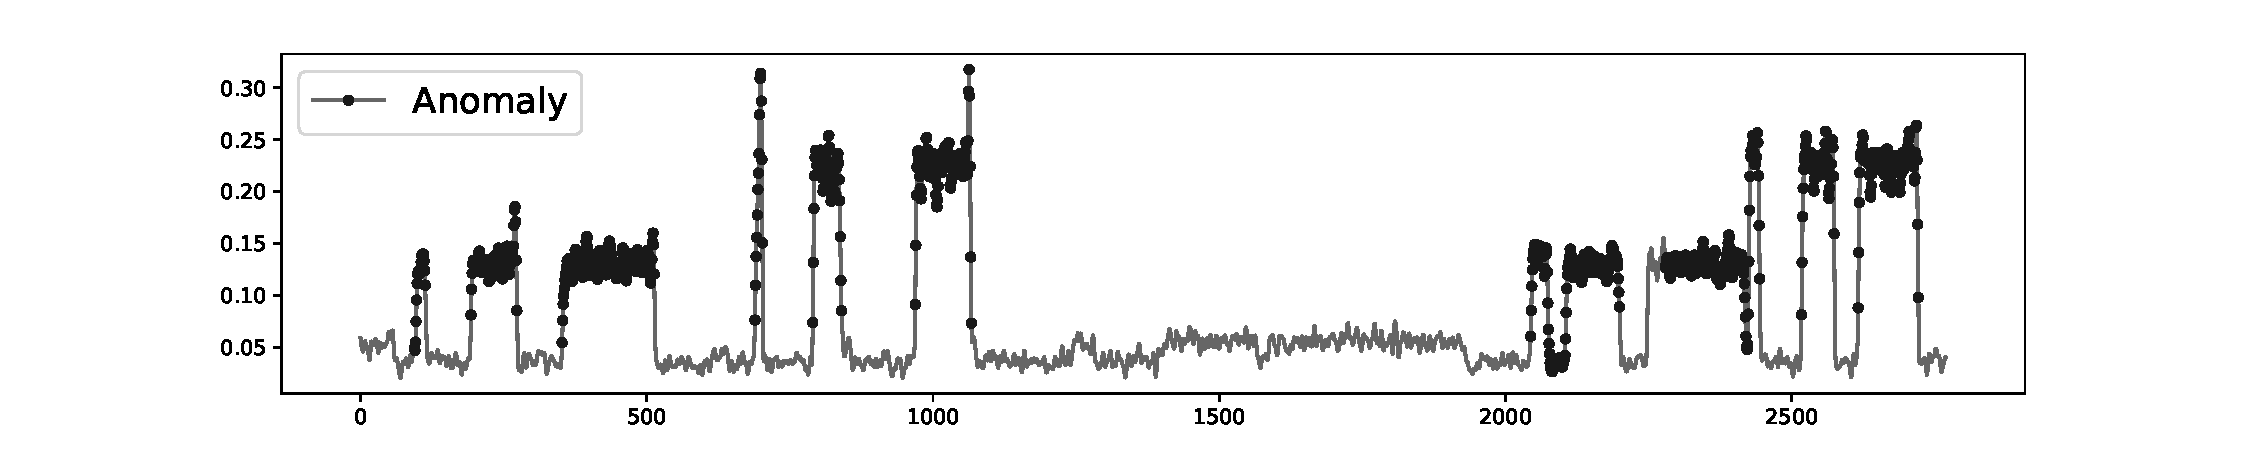
\includegraphics[width=0.48\textwidth]{gfx/chap4/scenario5.pdf}\label{scenario6}}
     \subfloat[][]{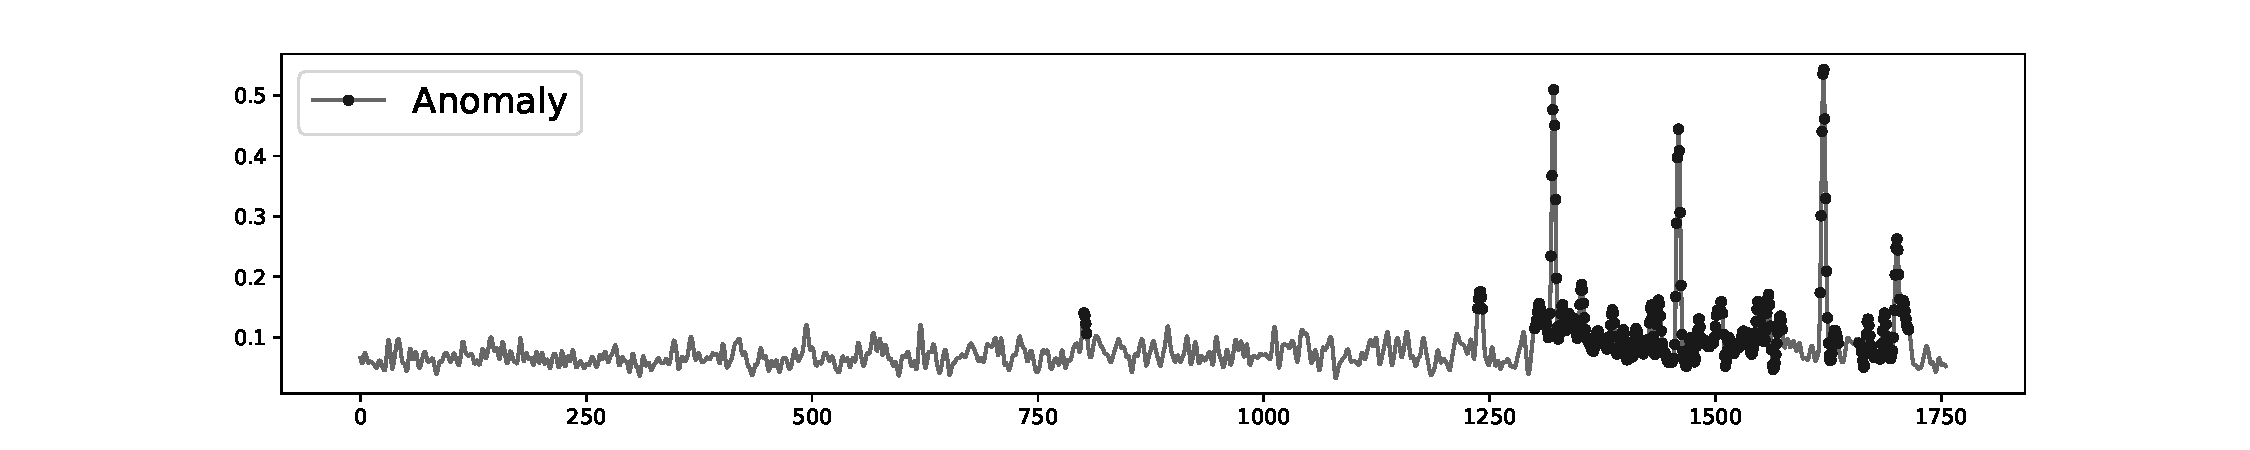
\includegraphics[width=0.48\textwidth]{gfx/chap4/scenario6.pdf}\label{scenario8}}
     \caption{Detected anomalies injected for scenarios (a) 5 and (b) 6.}
     \label{scenarios}
\end{figure*}


\begin{table}[!b]
\centering
\caption{F1 scores from production cloud metric data.}
\begin{tabular}{l|cc}
\hline
\begin{tabular}[c]{@{}l@{}}Service ID\end{tabular} & Donut & Metano \\ \hline
1                                                             & 0.72  & 0.90   \\
2                                                             & 0.26  & 0.4    \\
3                                                             & 0.67  & 0.86   \\ \hline
\end{tabular}
\label{tab:resultsproduction}
\end{table}

\begin{figure*}[!t]
     \centering
     \subfloat[][]{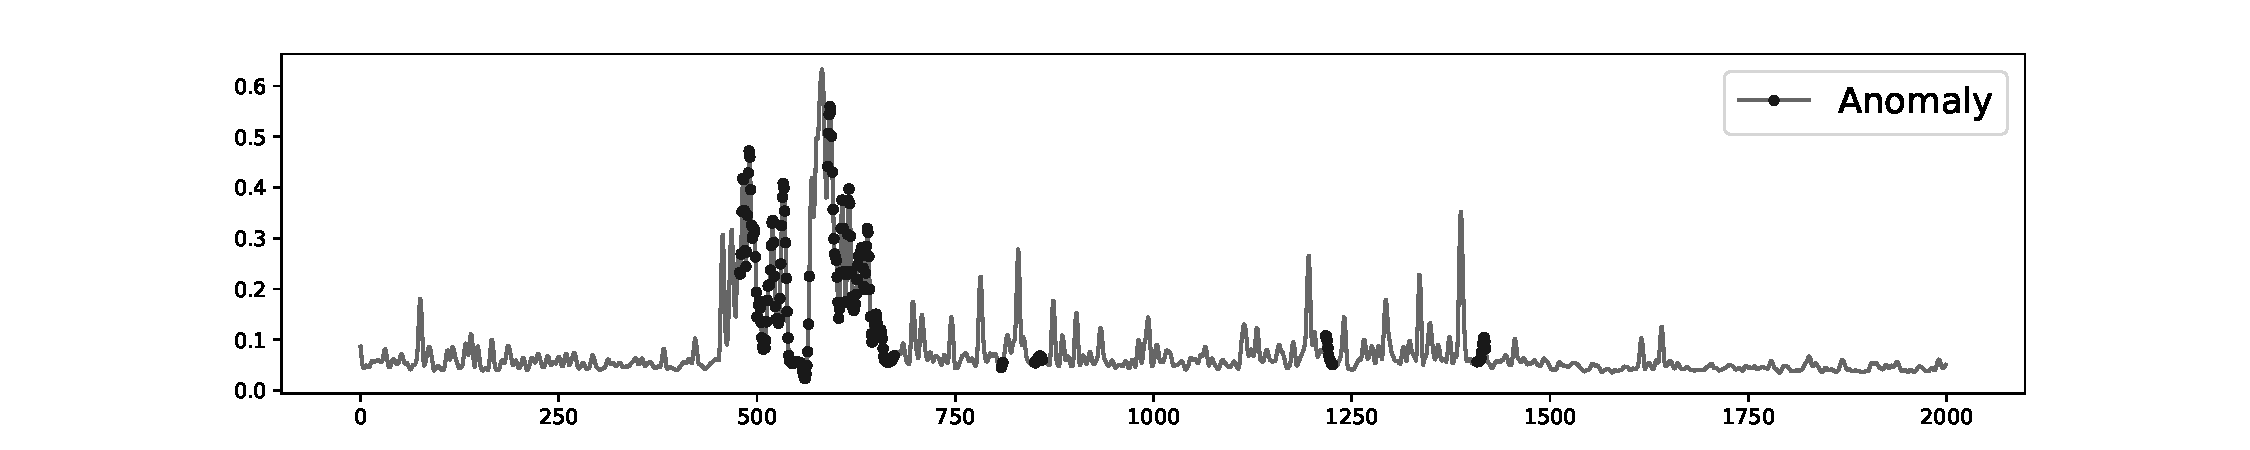
\includegraphics[width=1.0\textwidth]{gfx/chap4/donut1.pdf}\label{fig:donutresults}}
     \\
     \subfloat[][]{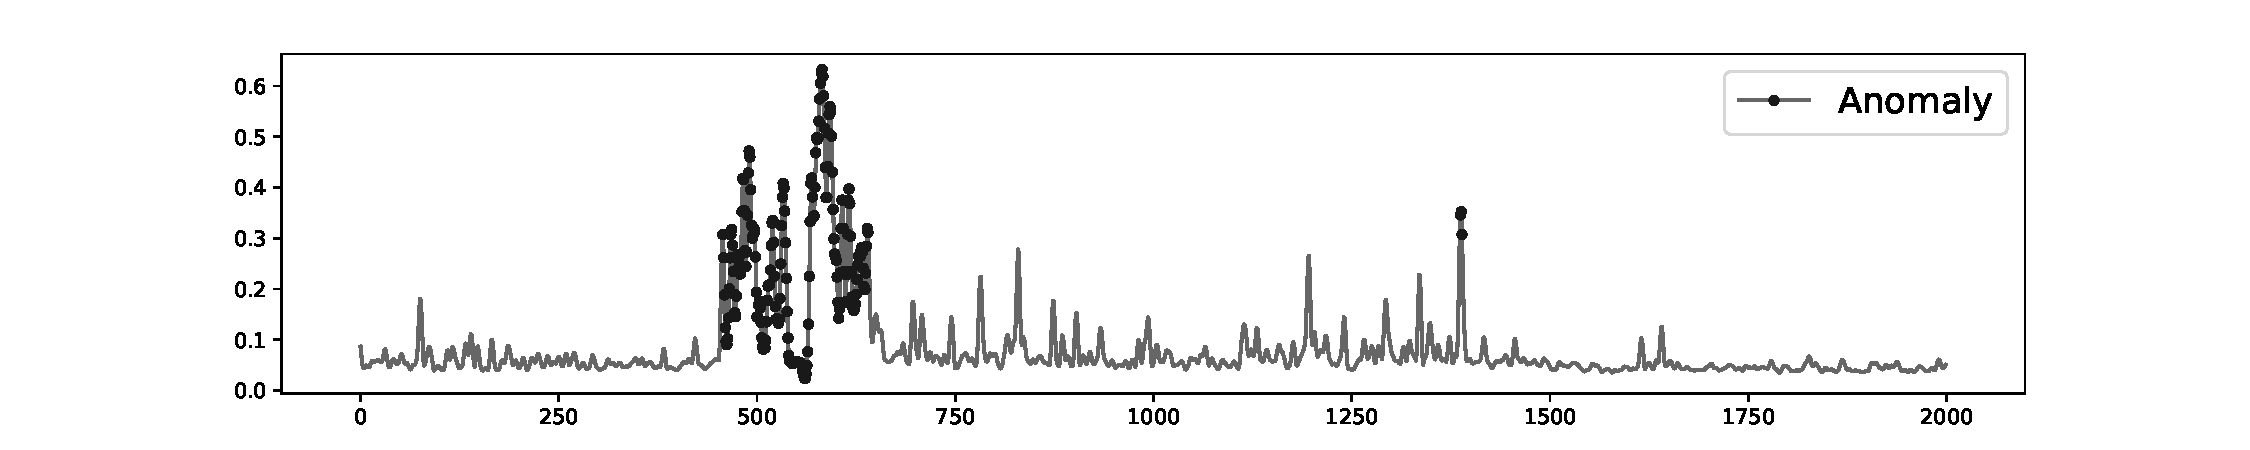
\includegraphics[width=1.0\textwidth]{gfx/chap4/vaelstm1.pdf}\label{fig:vaelstmresults}}
     \caption{Example of performed anomaly detection on the production data for one endpoint. (a) Donut, (b) Metano.}
     \label{fig:productionplotresults}
\end{figure*}

% \begin{figure*}[!t]
% \minipage{0.49\textwidth}
%   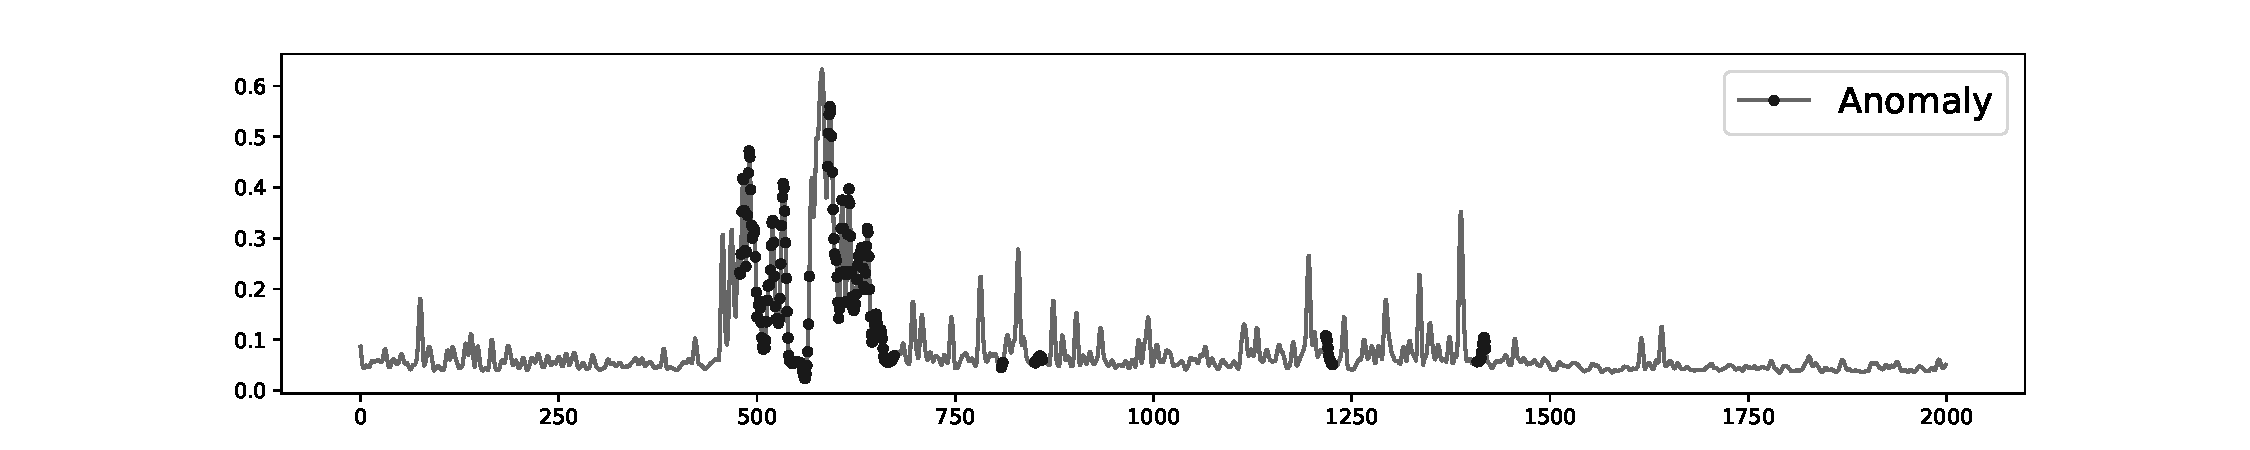
\includegraphics[width=1.0\textwidth]{gfx/chap4/donut1.pdf}\label{fig:donutresults}
% \endminipage\hfill
% \minipage{0.49\textwidth}
%   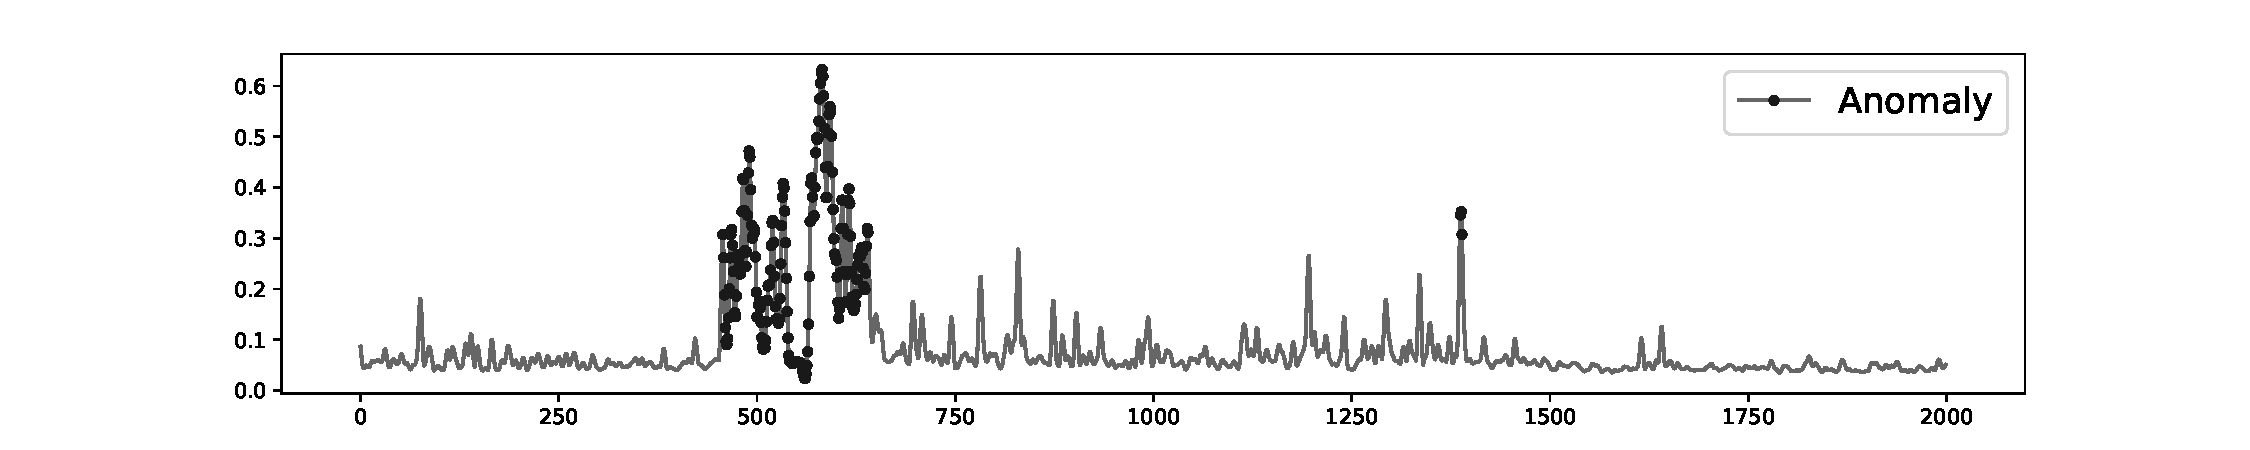
\includegraphics[width=1.0\textwidth]{gfx/chap4/vaelstm1.pdf}\label{fig:vaelstmresults}
% \endminipage
% \caption{Example of performed anomaly detection on the production data for one endpoint. (a) Donut, (b) Metano.}
% \label{fig:productionplotresults}
% \end{figure*}


\noindent\textbf{Production cloud data.} 
In the production data, in contrast to the microservice testbeds, we observed a higher noise. We show the results in Table~\ref{tab:resultsproduction}. The method has a good performance. However, decreases in the F1 scores were observed for both Metano and Donut for the production data, mainly owing to the high noise in the data. We illustrate the detection of anomalies on one production endpoint in Figure~\ref{fig:productionplotresults}. The plots show that 
Metano produces more stable predictions, while Donut has a larger number of FPs between the 750-th and 1500-th points in the time series. The analysis of the data points and method show that Metano leads to fewer FPs mainly owing to the noise handling techniques implemented in Metano, i.e., the tolerance module and increased model capacity.

\begin{figure}[!t]
\centerline{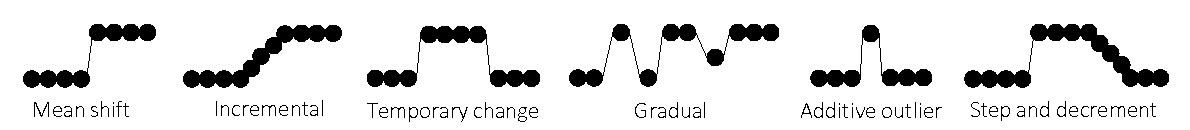
\includegraphics[width=1.0\textwidth]{gfx/chap5/patterns.pdf}}
\caption{Example of predefined patterns.}
\label{figpredefinedpatterns}
\end{figure}

Owing to the small number of production-system errors in the data, we injected several types of anomalies to further test the described method. We defined seven types of common anomalies, samples from normal distributions with different means, additive outlier, mean shift, step and decrement, incremental, temporary change, and gradual. Some of the types of anomalies are shown in Figure~\ref{figpredefinedpatterns}.

\begin{table}[htbp]
\centering
\caption{Robustness of Metano for detection of injected anomalies in production data.}
\begin{tabular}{ll}
\hline
Pattern name             &Parameters  \\ \hline
Additive\ outlier        &$RTi>0.25$   \\

Normal\_mean                          &$RTi>0.2$         \\

Temporary\ change                      &$RTi>0.25$          \\ 

Gradual                       &$RTi>0.3,\ size>10$\\ 

Mean\ shift                         &$RTi>0.2$\\

Step\ and\ decrement                      &$RTi>0.3,\ size>10$\\

Incremental                        &$RTi>0.3,\ size>10$ \\

\hline
\end{tabular}\label{tablevaeres}
\end{table}

To analyze the robustness of the algorithm, we evaluated it for several different augmentations of the original patterns, including translation, increasing the response time (e.g., $RTi=0.2$ implies setting the response time of the event to 0.2 of the maximum value), and change in the size of the anomaly (e.g., in gradual increase, $size=10$ implies that the increase from amplitude A to amplitude B is gradual over 10 events/data points). Table\ref{tablevaeres} shows the aggregated results. It summarizes the different anomaly patterns and needed minimum values for the parameters $size$ and $RTi$ that lead to detection of the corresponding anomaly type. 

\noindent\textbf{Sockshop microservice testbed.}
In this experiment, we slightly modified the input of the method to support multi-variate time series data (CPU, memory, network traffic, and response time). The method is designed for univariate time series data, as previously mentioned. However, with slight changes in the dimensionality of the input, we utilize the method to identify the root cause with anomaly detection. We computed the reconstruction errors for each of the time series.
For each fault injected in a service, we train the autoencoder with normal data and test with the anomalous data. A larger error of a particular metric compared to other metrics indicates that it has a higher probability to be the cause of the anomaly. 

Table~\ref{tabresultssockshop} shows the results of our method on different microservices and faults, in terms of precision for successfully predicting the anomaly and root cause. Our method achieve good performances in different services and faults, except for the service orders with the fault memory leak and network delay. This occurs because (1) orders is a computation-intensive service, (2) we heavily exhaust its resource memory in our fault injection, and (3) fault memory leak issues manifest as both high memory usage and high CPU usage. As our method targets the root cause, which manifests with a significant deviation in the causal metric, the accuracy decreases when the root cause manifests in multiple metrics. On average, our system achieves a precision of 94.75\%. 


\begin{table}[htbp]
\centering
\caption{Accuracy performance of Metano on Sockshop microservice testbed data.}

\begin{tabular}{lllll}
\hline
Service       & Orders & Catalogue & Carts & User \\ \hline
CPU hog       & 1.0    & 0.96      & 0.83  & 1.0  \\ 
Memory leak   & 0.66   & 1.0       & 1.0   & 1.0  \\ 
Network delay & 0.83   & 0.93      & 0.91  & 1.0  \\ \hline
\end{tabular}\label{tabresultssockshop}
\end{table}


% Further, in Figure \ref{vaeres1} and \ref{vaeres2} we visually illustrate some of the patterns detected in the series. The algorithm successfully detects the three types of anomalies injected. We note that the model was able to capture the multiple data distributions and shifts that appear early in both time series. Therefore it produced very small amount of FP.



% \begin{figure*}[htbp]
%      \centering
%      \subfloat[][]{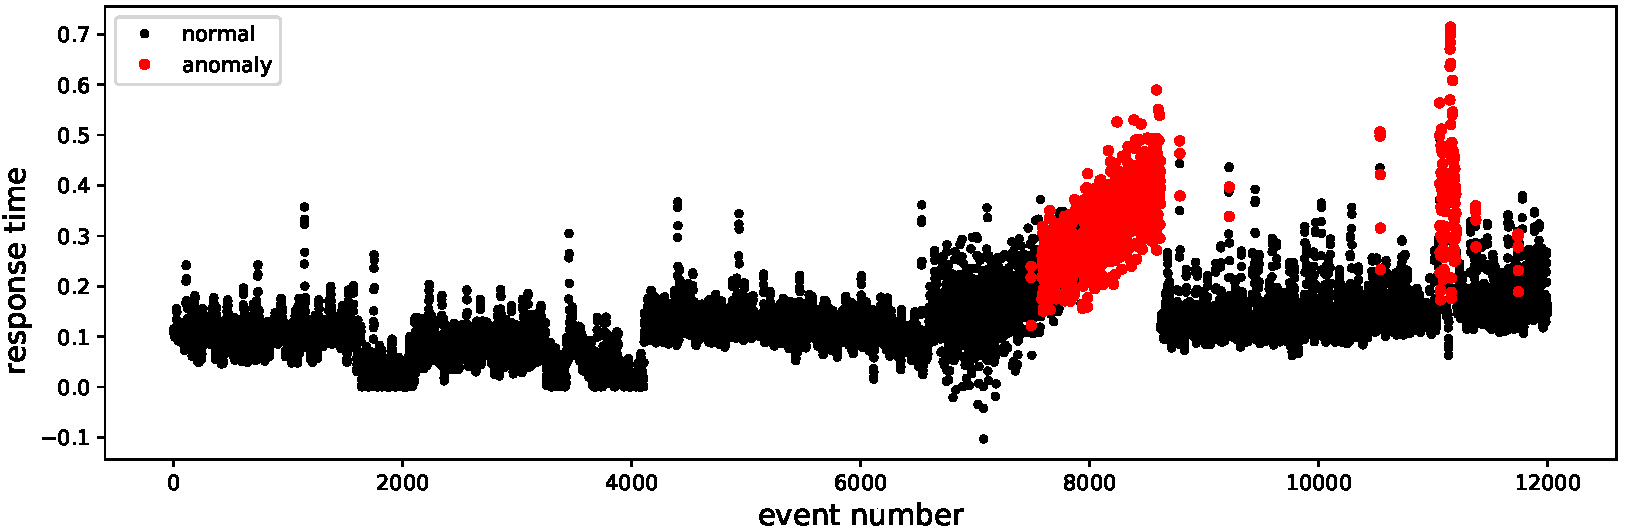
\includegraphics[width=1.0\textwidth]{gfx/chap5/vaeres1.pdf}\label{vaeres1}}
%      \\
%      \subfloat[][]{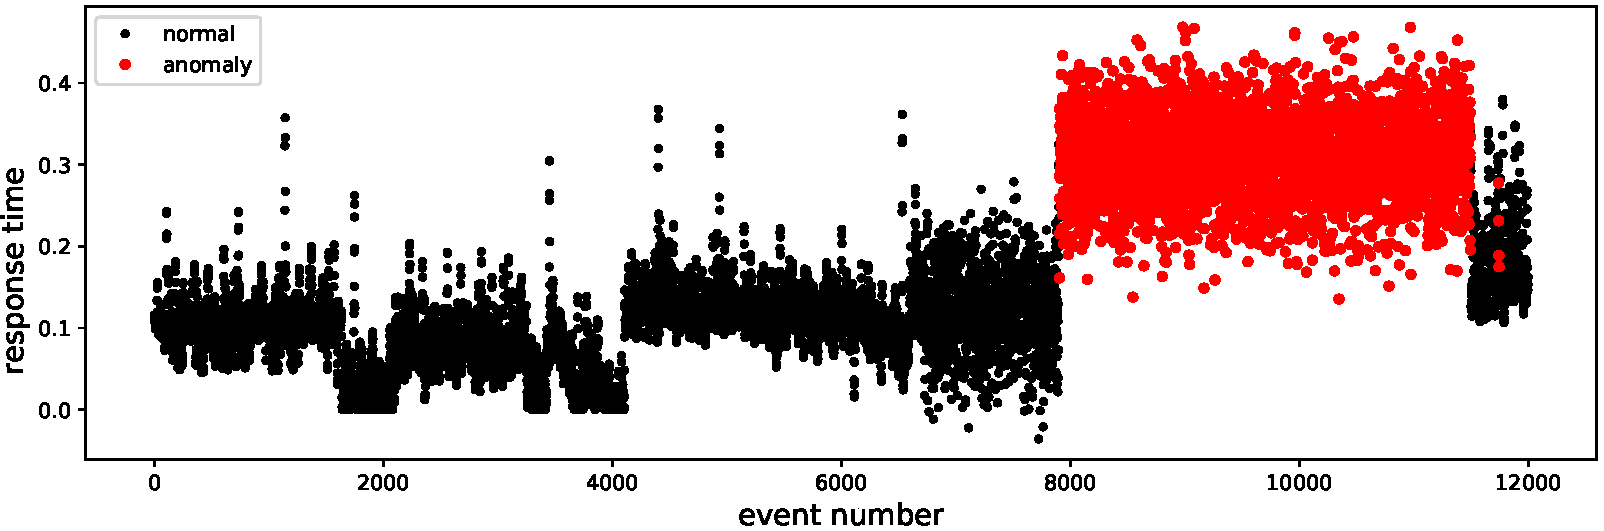
\includegraphics[width=1.0\textwidth]{gfx/chap5/vaeres2.pdf}\label{vaeres2}}
%      \caption{Example of successfully detected anomalies injected in \{host\}/ v1/\{p\_id\}/ cs/limits. Gradual and mean shift anomalies are injected in (a) and (b) respectively.}
%      \label{vaeres}
% \end{figure*}

\textbf{Faulty pattern classification}\label{resultspr}
The module can be evaluated separately from the rest of the solution, as data and predefined patterns as described. 
The dataset consists of 15 different types of patterns similar to those in Figure~\ref{figpredefinedpatterns}. In practice, the user can define patterns.

We evaluated the algorithm to analyze the performance and its limits according to the level of noise in the signal and  accuracy of classification. We achieved an accuracy of 100\% in data without additional noise and accuracies of 80\% and 48\% when Gaussian noise was added with $\sigma=0.05$ and $\sigma=0.1$, respectively. The CNN model accurately classifies the tested anomaly patterns, with an expected lower accuracy obtained in noisy patterns. For comparison, patterns recognizable by the human eye had noise levels up to approximately $\sigma=0.05$.

\subsubsection{Performance evaluation}
In large production systems, high performances of the model in training and prediction time are desirable. In this regard, we evaluate the performance of the approach. We show the results for training times in Table~\ref{perf_table1}. The training time scales linearly with the size of the time series (in number of windows). In the test-time prediction, we achieve a performance of 0.22 ms per predicted window of points (when $w=32$). The prediction times can differ with the reduction or expansion of the window size, but are still reasonably small for production usage within the limit below $10 ms$~\cite{nedelkoski2019anomaly}.

\begin{table}[htbp]
\centering
\caption{Performance evaluation of Metano in the training phase.}
\label{perf_table1}
\begin{tabular}{ ll}
\hline
\#windows  &s\\ \hline
10000	&283.9\\
5000    &148.2\\
2000	&58.56\\
1000	&31.33\\ \hline
\end{tabular}
\end{table}


\section{Related work} \label{related_work}
Anomaly detection for time series data has been extensively studied in academia and industry over the past years on different types of data. Machine learning approaches can be divided into two general categories~\cite{schmidt2018iftm}, supervised \cite{Breiman2001, joshi2001mining, joshi2002predicting, chawla2004special} and unsupervised \cite{fichtenberger2013bico,kanungo2002efficient, liu2008isolation, manevitz2001one}. The supervised methods have a limited practical usage as obtaining labels in production systems is costly and often infeasible, as described in \autoref{ch:background:sec:anomalydetection:subsec:supervised}. In the literature, the unsupervised time series anomaly detection methods are categorized into two types, deterministic and stochastic.

\textbf{Deterministic models}~\cite{malhotra2015long,filonov2016multivariate,vallis2014novel,donut,netflix,vrushali2016anomaly,Hundman:2018:DSA:3219819.3219845}. 
Several algorithms have been developed in the industry. Among them, the Netflix's robust principle component analysis (RPCA) method~\cite{netflix} and Twitter's anomaly detection~\cite{vallis2014novel}, where the underlying algorithm is referred to as seasonal hybrid ESD (S-H-ESD), which builds upon the Generalized ESD test for detecting anomalies, are most prominent. Similar ideas have been reported. For example, Vallis et al.~\cite{vallis2014novel} proposed a novel approach, based on an extreme studentized deviate (ESD) test, for detecting anomalies in long-term time series data. The approach requires detection of the trend component. Because these algorithms typically have simple assumptions for applicable metric time series (KPIs), expert's efforts need to be involved to pick a suitable detector for a given KPI, and then fine-tune the detector's parameters based on the training data. Simple ensemble of these detectors do not help much either according to~\cite{liu2015opprentice}. As a result, these detectors see only limited use in the practice. 

To address the large volumes of data produced by large systems, deep learning techniques are increasingly investigated because of their success in various domains. Malhotra et al.~\cite{malhotra2015long} used stacked recurrent hidden layers to enable learning of higher-level temporal features. They presented a model of stacked LSTM networks for anomaly detection in time series. A network was trained on nonanomalous data and used as a predictor over a number of time steps. Furthermore, Hundman et al. \cite{Hundman:2018:DSA:3219819.3219845} showed the use of LSTMs for spacecraft anomalies on telemetry data. Vrushali et al.~\cite{vrushali2016anomaly} in their paper on an anomaly-based intrusion detection system using neural networks show that these models can be used to detect various network attacks where the aim is to identify those attacks with the support of a supervised neural network. Although LSTMs-based methods can address the temporal dependence of time series, they are deterministic without stochastic variables. In our particular case, owing to the high noise they did not perform well (see~\autoref{metrics:evaluation}).

\textbf{Stochastic-based models}~\cite{fraccaro2016sequential,zong2018deep,park2018multimodal}. 
Zong et al.~\cite{zong2018deep} presented a deep autoencoding Gaussian mixture model (DAGMM) for unsupervised anomaly detection. The model utilizes a deep autoencoder to generate a low-dimensional representation and reconstruction error for each input data point, which is further fed into a Gaussian
mixture model (GMM). Instead of using decoupled two-stage training and standard expectation-maximization (EM) algorithm, DAGMM jointly optimizes the parameters of the deep autoencoder and mixture model simultaneously in an end-to-end manner, leveraging a separate estimation network to facilitate the parameter learning of the mixture model. The joint optimization, which well balances the autoencoding reconstruction, density estimation of the latent representation, and regularization, helps the autoencoder escape from less attractive local optima and further reduce the reconstruction errors, avoiding the need for pretraining. However, this method ignores the inherent temporal dependence of the time series. Previous studies suggest that, in general, stochastic variables can improve the performance of the RNN, because they can capture the probability distributions of the time series. Fraccaro et al.~\cite{fraccaro2016sequential} introduced stochastic RNNs, which combine a deterministic RNN and state space model to form a stochastic and sequential neural generative model. Xu et al. \cite{donut} showed the usability of VAEs for anomaly detection and triggering of timely troubleshooting problems on key performance indicator (KPI) data of Web applications (e.g., page views, number of online users, and number of orders). They proposed Donut, an unsupervised anomaly detection algorithm based on variational inference. Donut, at the time of evaluating Metano was considered as state-of-the-art method for anomaly detection using metric data from software systems, therefore used as a comparison method.

Compared to the above approaches, Metano is a variational RNN, which merges VAE and GRU so that the temporal dependence and stochastics of the time series can be explicitly modeled. Moreover, the inclusion of preprocessing and postprocessing with autonomous threshold selection and tolerance module improves the performance by reducing the number of false alarms. 

\section{Chapter summary}
Despite the plethora of methods and long-lasting research on time series anomaly detection, we discussed the few challenges of the task for system metric data. They include the high noise, several frequencies and distributions that reflect the normal system behavior, and recognition of patterns of anomalies.

To mitigate these challenges, we presented Metano, an approach that combines several deep learning models with pre- and postprocessing modules. We demonstrated the advantages of combining GRUs with VAEs, two deep learning models, for learning both stochastic and sequential properties of the time series data generated by distributed software systems. This is a part of the core anomaly detection model. Furthermore, we discussed the importance of the false alarm reduction logic together with the description of the recognized anomaly patterns. All proposed parts of Metano are designed to improve the administration with a small number of hyper-parameters. 
Our investigation on experimental and real-world production data showed that the approach reaches comparable to state of the art F1-scores with an average of 0.85, prediction time smaller than 10 ms, and robust classification of detected anomalies. The data were generated by two experimental microservice applications and planet-scale cloud infrastructure. Overall, we find comparable to state-of-the-art results on time series data.

Nevertheless, the largest drawback for metrics is that they contain only a limited view of the system and are system/service-scoped, which hinders the understanding except inside a particular system/service on a high level. Moreover, metrics do not provide semantic information about the anomalies, which can be found in logs and traces.
Therefore, in the next chapters, to provide a complementary and unified anomaly detection, we also analyze and present solutions in anomaly detection from log and trace data.